%\documentclass[aip,jcp,amsmath,twocolumn,floatfix,reprint,fleqn]{revtex4-1}
\documentclass[aip,jcp,amsmath]{revtex4-1}
\usepackage{amsmath}
\usepackage{color}
\usepackage{txfonts}
\usepackage{mathrsfs}
\usepackage{dcolumn}
\usepackage{bm}
\usepackage{graphicx}
\usepackage{here}
\usepackage{longtable}
\usepackage{rotating}
%\usepackage {threeparttable}
%\usepackage[dvipdfmx]{graphicx}
\newcommand{\half}{{\textstyle \frac{1}{2}}}
\newcommand{\quarter}{{\textstyle \frac{1}{4}}}
\newcommand{\centerc}[1]{\multicolumn{1}{c}{#1}}
\usepackage[pdfborder={0 0 0}]{hyperref}
\allowdisplaybreaks
\hypersetup{
    colorlinks,%
    citecolor=blue,%
    linkcolor=blue,%
    urlcolor=blue
}

\newcommand{\red}[1]{\textcolor{red}{#1}}
\newcommand{\myfnmark}[1]{\mbox{\textsuperscript{\normalfont #1}}}

\begin{document}

\title{\color{blue}
  A Multireference Coupeld-Eletron Pair Approximation combined with Complete-Active Space Perturbation Theory in Local Pair-Natural Orbital Framework}
\date{\today}
\author{Masaaki \surname{Saitow}}
\email{msaitow514@gmail.com}
\affiliation{Department of Chemistry, Graduate School of Science, Nagoya University, 1-5 Chikusa-ku, Nagoya, Aichi 464-8602, Japan}

\author{Takeshi \surname{Yanai}}
\affiliation{Department of Chemistry, Graduate School of Science and Institute of Transformative Bio-Molecules (WPI-ITbM), Nagoya University, 1-5 Chikusa-ku, Nagoya, Aichi 464-8602, Japan}
\affiliation{Japan Science and Technology Agency, PRESTO, 4-1-8 Honcho, Kawaguchi, Saitama 332-0012, Japan}

\begin{abstract}  
  %
  The Complete Active Space Second-order Perturbation Theory (CASPT2) has been one of the most widely used methods for caluclating the electronic structure of the multireference systems with semi-quantitative accuracy.
  %
  As a simple, yet higher-order approach, we have developed a hybrid theory of the CASPT2 and a multireference variant of the Coupled-Electron Pair Approximation (CEPA) in the fully-internally contracted framework.
  %
  In the newly developed theory (CEPT2), the external components of the wave functions, which usually give the most significant contribution to the dynamic correlation energy, are solve at the CEPA level while the rests are treated at the CASPT2 level.
  %
  Moreover, using an automatic expression and code generation technique, we have implemented the CASPT2 and CEPT2 approaches in the pair-natural orbital (PNO) framework to reduce their computational costs with respect to the number of atomic orbital (AO) basis.
  %
  To highlight the accuracy of the CEPT2 approach and to assess the errors caused by the PNO truncation, we have performed benchmark calculations on small- to medium-size molecules including dissociation of N${}_2$ molecule.
  %
  MADA-MADA
  
\end{abstract}

\maketitle

\section{Introduction}
%
Electronic structures that cannot be well approximated by a single Slater determinant are common in chemistry.
%
%Quantum chemical description of chemical reactions involving cleavage of covalent bonds is a very typical example
Electronic wave function of the low-spin open-shell states where there are multiple anti-ferromagnetically coupled electrons is a very typical example of such cases.\cite{NEESE2009526}
%
The electron correlation effect that plays an important role in these problems is often referred to as static correlation.\cite{doi:10.1021/cr2001417}
%
However, to obtain quantitave accuracy, it is often necessary to consider dynamic correlation which is the remaining component of the correlation effect.
%
The most stratghtforward way to take into account both types of correlation in a well-balanced manner is the multireference (MR) wave function theories\cite{MCSCFandMRCI2011,doi:10.1021/cr300500z} that are based on the multiconfigurational self-consistent field (CASSCF) reference function.\cite{roosa1980,Roos1987,ruedenbergmcscf1979}
%
Note that there are tremendous attempts to utilize the single-reference (SR) framework\cite{doi:10.1063/1.481769,doi:10.1063/1.1290609,doi:10.1021/jp056791e,doi:10.1021/acs.jctc.9b00456,doi:10.1063/1.4991020,doi:10.1063/1.5053605,doi:10.1063/1.5085314,doi:10.1021/acs.jctc.6b00137,doi:10.1063/1.5036542,doi:10.1002/jcc.25163} for capturing the static correlation effect.

%
%For achieving quantitative accuracy, it is often necessary to consider the remaining components of the electron correlation effect which is known as dynamic correlation.
%
%Amongst the MR wave function theories, the second-order perturbation expansions of the wave function (MRPT2) have been formulated in several different ways and implemented in most of common quantum chemistry program packages.
%
Amongst the MR wave function theories, the Second-order Complete-Active-Space Perturbation Theory (CASPT2) pioneered by Roos and coworkers\cite{doi:10.1021/j100377a012,doi:10.1063/1.462209} in early 90s have been used as a fundamental tool for achieving quantitative accuracy for systems of complicated electronic structure including organic molecules of doubly-excited nature\cite{doi:10.1063/1.2889385} and mono-\cite{doi:10.1021/ct900567c,doi:10.1021/acs.jctc.9b00166} and multinuclear\cite{Cramer2008,doi:10.1002/chem.201902766} transition metal complexes.
%
A newer variant of CASPT called N-Electron Valence-state Perturbvation Theory (NEVPT) was proposed by Angeli {\it et al.}\cite{angeliintroduction2001,angelin-electron2002,angelinew2006} using Dyall's zeroth-order Hamiltonian\cite{dyallthe1995} to overcome some of the shortcomings of CASPT approach.
%
As both approaches converge to the conventional second-order M\o ller-Plesset (MP2) perturbation theory\cite{MP2} in the SR limit, floating-point operations (FPOs) needed to calculate CASPT2 and NEVPT2 energies scale at least as O($c^2v^2$) for system with a fixed number of active molecular orbitals (MOs) where $c$ and $v$ represent the number of doubly-occupied and virtual MOs, respectively.
%
Before calculating CASPT2 energy, one has to solve the first-order amplitude equations and hence the memory or storage requirement scales also as O($c^2v^2$).
%
For a system with more active MOs, the prefactors of both memory and FPO requiremtns steeply increase because their working equations involve the reduced-density matrices (RDMs) of up to 4th order.
%
Therefore, routine application of CASPT2 methods to systems with more than 1,000 atomic orbital (AO) functions is often prohibited.

%
To improve the applicability of CASPT2 approach, numerous efforts have been including use of frozen-natural orbitals (FNOs)\cite{doi:10.1063/1.3157463,doi:10.1021/acs.jctc.5b00479} in the virtual space in conjunction with the Cholesky decomposition technique for reducing the costs of MO integral transformation\cite{doi:10.1063/1.2953696,doi:10.1021/ct9000284,doi:10.1021/ct700263h,doi:10.1021/ct900612k} and of the tensor-hyper-contraction-based (THC-) CASPT2.\cite{doi:10.1063/1.5037283}
%
The density-fitting (DF) or resolution-of-the-identity (RI) approximation has also been used for accelerating CASPT2 computation.\cite{ShioWerner2013}
%
Recently, Katz and Werner developed a CASPT2 approach in the so-called pair-natural orbital (PNO) framework, which has been coined PNO-CASPT2, and demonstrated its applicability to large, real-life MR systems composed of up to approximately 3,000 AO functions.\cite{:/content/aip/journal/jcp/145/12/10.1063/1.4963019,doi:10.1063/1.5097644}

%
The original concept of PNOs was already realized in 60s in order to accelerate the concergence of the configuration interaction (CI) expansions.\cite{:/content/aip/journal/jcp/40/12/10.1063/1.1725065,:/content/aip/journal/jcp/48/4/10.1063/1.1668917,:/content/aip/journal/jcp/42/3/10.1063/1.1696050,:/content/aip/journal/jcp/45/5/10.1063/1.1727841,meyer1971ionization,:/content/aip/journal/jcp/58/3/10.1063/1.1679283,meyer1971ionization,Ahlrichs1968_2}
%
Importantly, the PNO-based MRCI theory and the MR Coupled-Electron Pair Approximation (PNO-MCCEPA) using internally-contracted (IC) configuration functions were developed by Taylor\cite{:/content/aip/journal/jcp/74/2/10.1063/1.441186} and Staemmler {\it et al.},\cite{Staemmler1993} respectively.

%
The use of PNOs in the context of modern wave function theories was first introduced by Neese and coworkers in their local PNO-based (LPNO-) CEPA\cite{neeseefficient2009cepa} and Coupled-Cluster (LPNO-CC)\cite{neeseefficient2009,hansenefficient2011,doi:10.1021/ct100445s} methods implemented in Orca package.\cite{WCMS:WCMS1327}
%
The LPNO-CEPA/CCSD is applicable to systems composed of up to 2,000 AO basis which is far beyond the reach of canonical counterpart while reconvering almost 99.9 $\%$ of the canonical correlation energy.
%
Later they have developed a more sohisticated variant called domain-based LPNO-CC (DLPNO-CC) methods for large, real-life systems involving hundreds of atoms and thousands of AO functions.\cite{riplingeran2013,riplingernatural2013,pinskisparse2015,riplingersparse2016,doi:10.1063/1.4981521,dipayan2016}
%
The DLPNO scheme has been extended to MR wave function theories resulting in DLPNO-Mk-MRCCSD\cite{doi:10.1021/acs.jctc.5b00334,doi:10.1021/acs.jctc.7b01184,C8CP03577F} and DLPNO-NEVPT2\cite{:/content/aip/journal/jcp/144/9/10.1063/1.4942769} methods.
%
In a similar vein, variants of PNO-based reduced-scaling wave function methods have been developed by many research groups including PNO-LCC methods by Werner {\it et al.}\cite{doi:10.1021/ct500725e,wernersdecay,doi:10.1021/acs.jctc.7b00554,publ7820099,publ8744633,publ9370681,publ9337428} and a variant of PNO-CC method and PNO-based theories for the excited states by H\"attig {\it at al.}\cite{doi:10.1080/00268976.2013.794314,doi:10.1080/00268976.2016.1263762,doi:10.1063/1.4972001,QUA:QUA24098,C4CP03502J,:/content/aip/journal/jcp/135/7/10.1063/1.3624370,:/content/aip/journal/jcp/135/21/10.1063/1.3664902,:/content/aip/journal/jcp/136/20/10.1063/1.4719981,:/content/aip/journal/jcp/139/8/10.1063/1.4819071} to only name a few.

%
%The IC-MRCI method and its size-consistency corrected variants often provides a much higher accuracy than CASPT2 for small molecules.
%The IC-MRCC methods pioneered by Simons and extended by K\"ohn {\it et. al} often provide a sophisticated treatment of electron correlation than the MRCI and the second-order perturbation theories.
%
%However, 

%Nowadays, developments of highly accurate reduced-scaling SR and MR wave function methods using PNOs have become an active field
In this paper, we report a hybrid of IC-MR-CEPA and CASPT2, which is conined CEPT2, as a higher-order, yet simple extenton to conventional CASPT2 method.
%
Even though the standard full of IC-MR-CEPA/0 lacks size-consistency, all the CEPA terms introduced are fully-connected and thus the near-size-consistent nature of CASPT2 is inherited to the CEPT2 model.
%
In CEPT2 method, the amplitudes of 2-external nature are solved at the MR-CEPA/0 level while the remaining amplitudes are treated at the CASPT2 level.
%
This way of combining two methods does not introduce any further terms involving 4-RDMs, which can be large data even for a medium-size CAS space, in comparison with the conventional CASPT2 approach.
%
Use of MR-CEPA ansatz for the 2-external subspaces introduces several terms involving 4-external MO integrals which may potentially make the whole computation quite demanding even for relatively small systems.
%
To overcome this issue, we introduce PNO expansion in the 2-external subspace in a similar vein to Ref. ~\onlinecite{:/content/aip/journal/jcp/145/12/10.1063/1.4963019}.
%
Derivation and implementation of our PNO-CASPT2/CEPT2 scheme have been achieved by an automatic code generation framework which was used in our previous works\cite{saitowmultireference2013,doi:10.1021/acs.jctc.5b00270} and has been extended to handle PNOs.

%
This paper proceeds as follows:XXXX

\section{Theory}\label{Sec:theory}

\subsection{Notations and Convention}
%
Throughout this paper, we use $ijkl\cdots$, $pqrs\cdots$ and $abcd\cdots$ to represent the doubly-occupied, active and virtual MOs, respectively, while the generic MOs are indicated by $wxyz\cdots$.
%
Derivation and the implementation of the working equations of the PNO-CEPT approach are based on the reduced spin-free excitation operators\cite{PhysRevA.43.3392,PhysRevA.41.2391,doi:10.1063/1.448859,Kutzelnigg_Mukherjee1997}
%
\begin{align}
  &E^w_x = \sum_{\sigma=\{\alpha,\beta\}} a^{w\sigma}a_{x\sigma} \label{eq:e1} \\
  &E^{wx}_{yz} = \sum_{\sigma,\tau=\{\alpha,\beta\}} a^{w\sigma}a^{x\tau}a_{z\tau}a_{y\sigma} \label{eq:e2}
\end{align}
%
where $a^{w}$ ($a_w$) represents the Fermionic creation (annihilation) operator that acts on $w$-th spatial MO.
%
By using Eqs. (\ref{eq:e1}) and (\ref{eq:e2}), the Born-Oppenheimer Hamiltonian is given as
\begin{align}
  H=\sum_{wx} h_{wx} + \frac{1}{2}\sum_{wxyz} (wy|xz) E^{wx}_{yz}
\end{align}
%
where $h_{wx}$ and $(wy|xz)$ are one- and two-electron integrals.
%
The redundant internally-contracted basis (r-ICBs) that span the first-order interacting space (FOIS) are generated by applying the following eight types of excitation operators to the reference function ($|\Psi_0\rangle$):
%
\begin{align}
  E_{ij}^{ab},\ E_{pi}^{ab},\ E_{pq}^{ab} \label{eq:externalICB}
\end{align}
%
for the external subspaces,
%
\begin{align}
  \{E_{ip}^{aq},\ E_{ip}^{qa}\},\ E_{ij}^{pa},\ E_{pq}^{ra} \label{eq:semiinternalICB}
\end{align}
%
the semi-internal subspaces and
%
\begin{align}
  E_{ij}^{pq},\ E_{ip}^{qr} \label{eq:intternalICB}
\end{align}
%
for the internal subspaces.
%
The energy and residual equations involve an expectation value of a string of $E$-operators with respect to the reference such as $\langle\Psi_0|E^{pq}_{ab}E_{wx}^{yz}\cdots|\Psi_0\rangle$.
%
Such an expectation value is evaluated by invoking Wick's theorem for the $E$-operators and is reduced to a reduced-density matrix (RDM) composed only of active MO indices:
%
\begin{align}
  &D^{p}_{q} = \langle\Psi_0|E^{p}_{q}|\Psi_0\rangle  \\
  &D^{pq}_{rs} = \langle\Psi_0|E^{pq}_{rs}|\Psi_0\rangle
\end{align}
%
The r-ICBs are non-orthonornal and linearly-independent set of functions as a basis of FOIS.
%
Therefore, the amplitude equations of MR wave function methods are solved in linearly-independent and orthonormalized IC representation spanned by the non-redundant (nr-) ICBs:
%
\begin{align}
  |\Psi_{ij}^{ab}\rangle,\ |\Psi_{\rho i}^{ab}\rangle,\ |\Psi_{\rho}^{ab}\rangle 
\end{align}
%
for the external subspaces,
%
\begin{align}
  |\Psi_{\rho i}^{a}\rangle,\ |\Psi_{ij}^{\rho a}\rangle,\ |\Psi_{\rho}^{a}\rangle
\end{align}
%
the semi-internal subspaces and
%
\begin{align}
  |\Psi_{ij}^{\rho}\rangle,\ |\Psi_{i\rho}\rangle
\end{align}
%
for the internal subspaces where $\rho\tau\cdots$ are used to represent the eigenvectors of metric for each subspace (Eqs. (\ref{eq:externalICB}) -- (\ref{eq:intternalICB})).

\subsection{Brief Summary of PNO-CASPT2 Algorithm}

%
As we follow a similar vein to the original formalism by Katz and Werner,\cite{:/content/aip/journal/jcp/145/12/10.1063/1.4963019,doi:10.1063/1.5097644} we only outline the PNO-CASPT2 theory in this section.
%
In CASPT2 method, the generalized Fock operator is used as the zeroth-order Hamiltonian
%
\begin{align}
  F=\sum_{wx} f_{wx} E^x_w
\end{align}
%
where $f$ represents the generalized Fock matrix
%
\begin{align}
  &f_{wx} = (f_\text{core})_{wx} + \sum_{pq} \left[(wx|pq)-\frac{1}{2}(wp|xq)\right]D^p_q \\
  &(f_\text{core})_{wx} = h_{wx} + \sum_{i} [2(wx|ii)-(wi|xi)]. 
\end{align}
%
The PNO-CASPT2 wave function is defined as
%
\begin{align}
  |\Psi\rangle&=\sum_{ij}\sum_{a_{ij}b_{ij}} t_{a_{ij}b_{ij}}^{ij}|\Psi_{ij}^{a_{ij}b_{ij}}\rangle+\sum_{\rho i}\sum_{a_{\rho i}b_{\rho i}} t_{a_{\rho i}b_{\rho i}}^{\rho i}|\Psi_{{\rho i}}^{a_{\rho i}b_{\rho i}}\rangle \nonumber \\
  &+\sum_{\rho}\sum_{a_{\rho}b_{\rho}} t_{a_{\rho}b_{\rho}}^{\rho}|\Psi_{{\rho}}^{a_{\rho}b_{\rho}}\rangle + \sum_{\rho ij}\sum_{a_{ij}} t_{a_{ij}\rho}^{ij}|\Psi_{ij}^{\rho a}\rangle +\sum_{\rho i}\sum_a t_{a}^{\rho i}|\Psi_{\rho i}^{a}\rangle \nonumber \\
  &+\sum_{\rho}\sum_a t_{a}^\rho|\Psi_\rho^a\rangle + \sum_{\rho ij} t_{\rho}^{ij}|\Psi_{ij}^\rho\rangle+\sum_{\rho i} t_{\rho}^i|\Psi_{i}^\rho\rangle \label{eq:pno-caspt2}
\end{align}
%
in the nr-ICB which is constructed by orthonormalizing and canonicalizing the redundant r-ICBs.
%
For instance, an nr-ICB with double excitations to the active space, $\{\Psi^{\rho}_{ij}\}$, is related to its redundant counterpart as
%
\begin{align}
  |\Psi_{ij}^{\rho}\rangle=\sum_{pq} C_{pq}^{\rho} |\tilde{\Psi}_{ij}^{pq}\rangle = \sum_{pq} C_{pq}^{\rho} E_{ij}^{pq} |\Psi_0\rangle
\end{align}
%
where the orthonormalization matrix, $\mathbf{C}$, is obtained by solving the generalized eigenvalue problem:
%
\begin{align}
  \sum_{rs}\langle\Psi_0|E_{pq}^{ij}FE_{rs}^{ij}|\Psi_0\rangle C_{rs}^\rho=E_{\rho ij}\sum_{rs}\langle\Psi_0|E_{pq}^{ij}E_{rs}^{ij}|\Psi_0\rangle C_{rs}^\rho. \label{eq:eigen-Vp2}
\end{align}

The PNO-CASPT2 amplitudes are determined by solving the residual equations
%
\begin{align}
  r^I&=\frac{\partial}{\partial t^I}\mathscr{F}_\text{PNO-CASPT2} \nonumber \\
     &=\sum_J \langle\Psi^I|F-\langle F\rangle|\Psi_J\rangle t^J-\langle\Psi^I|H|\Psi_0\rangle\rightarrow 0 \label{eq:caspt2-residua}
\end{align}
%
where $IJ$ represent one of the eight non-redundant subspaces of FOIS.
%
The Hylleraas-type energy functional for PNO-CASPT2 ansatz is given as
%
\begin{align}
  \mathscr{F}_\text{PNO-CASPT2}=\langle\Psi|H|\Psi_0\rangle+\langle\Psi_0|H|\Psi\rangle+\langle\Psi|F-\langle F\rangle|\Psi\rangle.
\end{align}
%
The amplitudes in the r-ICB representation ($\tilde{\mathbf{t}}$) can be obtained by back-transforming the nr-ICB counterpart ($\mathbf{t}$) as
%
\begin{align}
  \tilde{t}^{pq}_{ij} = \sum_{\rho} C_{pq}^\rho  t^{\rho}_{ij}.
\end{align}
%
In typical canonical CASPT2 implementation, the residua that correspond to Eq. (\ref{eq:caspt2-residua}) are evaluated in r-ICB representation using the $\tilde{\mathbf{t}}$ amplitudes, and then transformed into the nr-ICB representation as
%
\begin{align}
  r^{\rho}_{ij}=\sum_{\rho} C_{pq}^\rho \tilde{r}^{pq}_{ij}.
\end{align}
for the $\{\Psi^{\rho}_{ij}\}$ subspace.

%
In Eq. (\ref{eq:pno-caspt2}), the PNOs are introduced only in the external subspaces and a semi-internal subspace spanned by $\{\Psi_{ij}^{\rho a_{ij}}\}$ function.
%
Since the PNOs for $\{\Psi_{\rho}^{a_{\rho}b_{\rho}}\}$ and $\{\Psi_{\rho i}^{a_{\rho i}b_{\rho i}}\}$ subspaces are dependent also on the nr-ICBs, in the PNO-CASPT2 implementation, one cannot back-transform the external amplitudes ($\mathbf{t}$) and the residua ($\mathbf{r}$) into the r-ICB representation while taking advantage of compactness of the PNO space.
%
Therefore, in our PNO-CASPT2 implementation, we do not perform any back-transformation into the r-ICB representatation and the residua are constructed directly in the nr-ICB representation using the orthonormalized amplitudes.
%
Thee explicit formuals for the orthonormalized amplitudes are given in Appendix I.

%
The PNOs for $ij-$, $\rho i-$ and $\rho-$pairs are generated by diagonalizing the pair-densities for the corresponding pairs:
%
\begin{align}
  &(D^{ij})_{ab}    =\langle\Psi_{ij}    |E^a_b|\Psi_{ij}    \rangle \ \ \ \ (\text{for}\ \{\Psi_{ij}^{ab}\}\ \text{subspsace}) \label{eq:Dij}\\
  &(D^{\rho i})_{ab}=\langle\Psi_{\rho i}|E^a_b|\Psi_{\rho i}\rangle \ \ \ \ (\text{for}\ \{\Psi_{\rho i}^{ab}\}\ \text{subspsace})\\
  &(D^{\rho})_{ab}  =\langle\Psi_{\rho}  |E^a_b|\Psi_{\rho}  \rangle \ \ \ \ (\text{for}\ \{\Psi_{\rho}^{ab}\}\ \text{subspsace})\\  
\end{align}
%
For $\{\Psi_{ij}^{\rho a_{ij}}\}$ subspace, we use the $ij-$PNOs obtained as eigenfunctions of Eq. (\ref{eq:Dij}).
%
Those PNOs with smaller occupation numbers than a user defined threshold are screened out.
%
The PNO truncation error for a pair is estimated by taking difference between full and truncated semi-local (SL-) CASPT2-D pair-energies.
%
\begin{align}
  &e_{ij}=\langle\Psi_0|H|\Psi_{ij}\rangle \\
  &e_{\rho i}=\langle\Psi_0|H|\Psi_{\rho i}\rangle \\
  &e_{\rho}=\langle\Psi_0|H|\Psi_{\rho}\rangle \\  
\end{align}
%
Moreover, only those pairs with pair-energy larger than a given threshold proceeds to the iterative PNO-CASPT2/CEPT2 step.
%
The SL-CASPT2-D pair-functions are used for defining the pair-densities
%
\begin{align}
  &|\Psi_{ij}\rangle=\sum_{ab}\frac{(ia|jb)}{F_{ii}+F_{jj}-\epsilon_a-\epsilon_b}\ E_{ij}^{ab}|\Psi_0\rangle \\
  &|\Psi_{\rho i}\rangle=\sum_{ab}\frac{\langle\Psi_{\rho i}^{ab}|H|\Psi_0\rangle}{F_{ii}-e_\rho-\epsilon_a-\epsilon_b}\ \sum_{p} C_p^\rho E_{ip}^{ab}|\Psi_0\rangle \\
  &|\Psi_{\rho}\rangle=\sum_{ab}\frac{\langle\Psi_{\rho}^{ab}|H|\Psi_0\rangle}{e_\rho-\epsilon_a-\epsilon_b}\ \sum_{pq} C_{pq}^\rho E_{pq}^{ab}|\Psi_0\rangle.
\end{align}
%
The numerators in the SL-CASPT2-D amplitudes involve 2-external two-electron integrals and hence this part will be a computational bottleneck in a whole PNO-CASPT2 computation.
%
In our current implementation, we generate a full set of canonical 2-external integrals using the resolution-of-the-identity (RI) approximation and store them on disk.
%
This choice limits the applicability of our PNO-CASPT2 only up to systems composed of not more than 2,000 AO functions.
%
To overcome such a difficulty, domain truncation should be introduced in the RI 3-index integral generation and the final 2-external integral construction steps as done in the original PNO-CASPT2 implementations,\cite{:/content/aip/journal/jcp/145/12/10.1063/1.4963019,doi:10.1063/1.5097644} in the DLPNO-CC and NEVPT2 algorithms by Neese and coworkers\cite{riplingeran2013,riplingernatural2013,pinskisparse2015,riplingersparse2016,doi:10.1063/1.4981521,:/content/aip/journal/jcp/144/9/10.1063/1.4942769,dipayan2016,doi:10.1063/1.5027114} and in the PNO-LCC programs by Werner {\it et al.}.\cite{doi:10.1021/ct500725e,doi:10.1021/acs.jctc.5b00843,wernersdecay,doi:10.1021/acs.jctc.7b00554}

%
In the canonical CASPT2 implementation, the nr-ICBs are constructed as eigenfunctions of diagonal blocks of the zeroth-order Hamiltonian by solving the generalized eigenvalue problems akin to Eq. (\ref{eq:eigen-Vp2}) for all the eight subspaces.
%
Therefore, programming the residua (Eq. \ref{eq:caspt2-residua}) of diagonal blocks in the first term is quite simple.
%
However, in the PNO-based counterpart, all the matrix blocks involving at least one DOMO index should be programmed, leading to a drastic increase in the number of terms that should be derived and programmed.
%
To this end, we extended our code generator framework\cite{femto,saitowmultireference2013,doi:10.1021/acs.jctc.5b00270} such that codes for the PNO-based tensor contractions can also be generated.
%
In our program, the PNO-CASPT2 residul equations are solved by the preconditioned conjugate gradient (PCG) algorithm.

%
We have also implemented real\cite{ROOS1995215} and imaginary\cite{FORSBERG1997196} shifts in our PNO-CASPT2 program in the same way as the canonical CASPT2 program.
%
The conventional formulation of the imaginary shifts is based on the diagonality in the diagonal blocks of zeroth-order Hamiltonian matrix in FOIS which is not satisfied if the DOMOs are localized.
%
Therefore, in our PNO-CASPT2 implementatin, the off-diagonal elements in the diagonal blocks are discarded, leading to a semi-canonical imaginary shift.

\subsection{The Coupled-Electron Pair Perturbation Theory}\label{Subsec:cept2}
%
%Being based on Fink's zeroth-order Hamiltonian\cite{FINK2006461,FINK200939} which does not involve any excitations that change the total number of electrons in the doubly-occupied, active and virtual orbital spaces, the so-called Retaining the Excitation degree Perturbation Theory (REPT) is obtained. 
%
%When applied to closed-shell single-reference function, the second-order REPT (REPT2) converges to the CEPA/0 Doubles (CEPA/0(D)) or alternatively known as Linearized Coupled-Cluster Doubles (L-CCD). 
%
%The MR variants of REPT in the Matrix Product State (MPS) and in the partially IC representations

%
In the PNO-CEPT2 ansatz, we minimize the following energy functonal
%
\begin{align}
  &\mathscr{F}_\text{PNO-CEPT2} = \mathscr{F}_\text{PNO-CEPA/0}^\text{ext}+\mathscr{F}_\text{PNO-CASPT2}-\mathscr{F}_\text{PNO-CASPT2}^\text{ext} \label{eq:F-CEPT2} \\
  &\mathscr{F}_\text{PNO-CEPA/0}^\text{ext} = \langle\Psi^\text{ext}|H-E_0|\Psi^\text{ext}\rangle \label{eq:F-CEPA/0} \\
  &\mathscr{F}_\text{PNO-CASPT2}^\text{ext} = \langle\bar{\Psi}^\text{ext}|H|\Psi_0\rangle + \langle\Psi_0|H|\bar{\Psi}^\text{ext}\rangle+\langle\bar{\Psi}^\text{ext}|F-\langle F\rangle|\bar{\Psi}^\text{ext}\rangle \label{eq:F-CASPT2}
\end{align}
%
where $\bar{\Psi}^\text{ext}$ represents the external part of the wave function
%
\begin{align}
  |\Psi^\text{ext}\rangle&=|\Psi_0\rangle+|\bar{\Psi}^\text{ext}\rangle \nonumber \\
  &=|\Psi_0\rangle+\left[\sum_{ij}\sum_{a_{ij}b_{ij}} t_{a_{ij}b_{ij}}^{ij}|\Psi^{a_{ij}b_{ij}}_{ij} \right. \nonumber \\
    &+ \left.\sum_{\rho i}\sum_{a_{\rho i}b_{\rho i}} t_{a_{\rho i}b_{\rho i}}^{\rho i}|\Psi^{a_{\rho i}b_{\rho i}}_{\rho i}\rangle + \sum_{\rho}\sum_{a_{\rho}b_{\rho}} t_{a_{\rho}b_{\rho}}^{\rho}|\Psi^{a_{\rho}b_{\rho}}_{\rho}\rangle\right].
\end{align}
%
By differentiating the above functional with respect to the amplitudes, one obtains the PNO-CEPT2 residual equations as
%
\begin{align}
  &r^{E}=\langle\Psi^{E}|H|\Psi_0\rangle+\sum_{E^{'}}\langle\Psi_E|H-E_0|\Psi_{E^{'}}\rangle t^{E^{'}}+\sum_{A}\langle\Psi_E|F|\Psi_A\rangle t^A \rightarrow 0 \label{eq:CEPT-E} \\
  &r^{A}=\langle\Psi^{A}|H|\Psi_0\rangle+\sum_{E}\langle\Psi_A|H|\Psi_E\rangle t^E+\sum_{A^{'}}\langle\Psi_A|F-\langle F\rangle|\Psi_{A^{'}}\rangle t^{A^{'}} \rightarrow 0 \label{eq:CEPT-A}
\end{align}
%
where $\{E\}$ and $\{A\}$ represent the external and the remaining subspaces in FOIS, respectively.
%
If one evaluates the diagonal block for $\{\Psi_{\rho}^{a_{\rho}b_{\rho}}\}$ straightforwardly using Wick's theorem, there are two terms involving 4-body RDM whose size is approximately 32 gigabyte for systems composed of 16 active MOs.
%
To eliminate such expensive contractions, we employ a commutator-based transformation originally proposed by Angeli and coworkers\cite{angeliintroduction2001,angelin-electron2002,angelinew2006}
%
\begin{align}
  r_{a_\rho b_\rho}^{\rho} &= \sum_{\tau}\sum_{c_\tau d_\tau}\langle\Psi_{a_\rho b_\rho}^{\rho}|H-E_0|\Psi_{\tau}^{c_\tau d_\tau}\rangle t_{c_\tau d_\tau}^\tau \nonumber \\
  &= \sum_{\tau}\sum_{c_\tau d_\tau} \sum_{pqrs} C_{pq}^\rho \langle\Psi_0|E_{_{a_\rho b_\rho}}^{pq}(H-E_0)E_{pq}^{c_\tau d_\tau}|\Psi_0\rangle C_{rs}^\tau t_{c_\tau d_\tau}^\tau \nonumber \\
  &= \sum_{\tau}\sum_{c_\tau d_\tau} \sum_{pqrs} C_{pq}^\rho \langle\Psi_0|E_{_{a_\rho b_\rho}}^{pq}[H,E_{pq}^{c_\tau d_\tau}]|\Psi_0\rangle C_{rs}^\tau t_{c_\tau d_\tau}^\tau \label{eq:comm}
\end{align}
as we have also utilized in our previous works for developing an approximated FIC-MRCI variants with a DMRG reference function.\cite{saitowmultireference2013,doi:10.1021/acs.jctc.5b00270}
%
Note that both the CEPT2 and the CIPT2\cite{celanithe2004} methods use the energy functional of the similar form.
%
The only difference between them consists in the choice of the CEPA subspaces; in the CEPT2 ansatz the external configurations are treated at the CEPA level while in the CIPT2 method the CEPA functional is used for in subspaces with three active MO indices i.e, $\{\Psi_i^\rho\}$ and $\{\Psi_\rho^a\}$.

%
The second term in Eq. (\ref{eq:CEPT-E}) involves contractions of the 4-external exchange-type integrals with the 2-external amplitudes which is known as the most expensice terms in the canonical CC or CEPA implementations.
%
However, such terms are typically not a bottleneck any more if the virtual space is spanned by the PNOs.
%
Some of the PNO-CEPA terms involve the semi-joint pair-pair interactions and in the MR case these terms appear to be more invlved.
%
Apparently, in the single-reference limit, the PNO-CEPT2 energy and wave function converge to those of PNO-CEPA/0(D) wave function.

%
All the CEPA terms in Eq. (\ref{eq:CEPT-E}) are {\it linked} in the sense that the amplitude is either directly or indirectly via 1-body density cumulant connected to the integral.
%
Therefore, as addressed in Ref. ~\onlinecite{AK74}, even for a super system ($A\cdots B$) composed of infinitely separated two subsystems ($A$ and $B$), no {\it unlinked} contractions appear.
%
This indicates that the CEPT2 extension does not violate the near-size-consistent character of original CASPT2 model.

%
Unlike CIPT2 which is designed to mitigate the intruder state problems typically stemming from the $\{\Psi_i^\rho\}$, $\{\Psi_\rho^a\}$ and the reference subspaces, in CEPT2, we use the CASPT2 ansatz for those subspaces.
%
In the single-reference case, it is known that the CEPA/0 energy can be irregular thus showing discontinuity in the potential energy surface.
%
To remedy this drawback, Taube introduced a regularization scheme which is closely related to the imaginary shift in the CASPT2 framework.\cite{doi:10.1063/1.3115467}
%
Therefore, we have implemented the real- and semi-canonical imaginary shifts and the Hylleraas corrections to minimize the errors caused by such shifts.

%
Our current implementation of the PNO-CEPT2 is still not of optimal form since only the 4-external terms and the 1-body terms such as those similar to the contractions from $\mathscr{F}_\text{PNO-CASPT2}^\text{ext}$ are fully evaluated in the PNO space.
%
All the remaining terms from $\mathscr{F}_\text{PNO-CEPA/0}^\text{ext}$, which involve either 4-internal integral or 2-external integral of semi-joint pair-pair interaction type,\cite{neeseefficient2009cepa,neeseefficient2009} are constructed in the canonical space using the back-transformed $\mathbf{t}$ amplitudes into the canonical space.
%
Therefore, we only demonstrate and benchmark the accuracy of the PNO-CEPT2 model for small- to medium-size molecules and the benchmarking the efficiency is beyond the scope of this manuscript.

\subsection{PNO-based Code Generation}
%
The automatic derivation and code generation technique has been a quite powerful strategy for developing and testing the novel wave function methods which often involve hundreds or thousands of tensor contraction terms to implement.\cite{CJanssen1991,doi:10.1021/jp034596z,SHirataTCE2004,SHirataTCE2006,doi:10.1080/00268970500275780,KoehnJCP2009_1,KoehnJCP2009_2,MHandKoehn2009,MHandKoehn2011,AK74,AK77,ShiozakiJCP2008,ShiozakiPCCP2008,ShiozakiJCP2009_1,ShiozakiJCP2009_2,doi:10.1063/1.4907717,doi:10.1063/1.4959029,doi:10.1002/jcc.24833,doi:10.1063/1.5001320,doi:10.1063/1.5048688,dattaa2011,doi:10.1063/1.3089302,doi:10.1063/1.3664729,PCMRCI2011}
%
To generate an efficient contraction code, each of the tensor contraction terms should be divided into a stream of binary contractions.
%
This is also the case for the code generations employing the PNOs spanning the virtual space.
%
Even though the global optimization scheme proposed by Hanrath and Engels-Putzka for developing the efficient higher-order CC codes\cite{hanrathan2010,engels-putzkaa2011} can also also used in such a context, in order to keep the generator tool relatively simple yet effective, we use a more heuristic strategy for forming the optimal binary contractions.

%
In canonical MO basis, typical contraction terms in the CEPT2 model read
%
\begin{align}
  r_{ab}^\rho &\leftarrow \frac{1}{4}\sum_\tau\sum_{pqrs}\sum_{c}(f_\text{core})_{ca} D^{pq}_{rs} t_{cb}^\tau C_{sr}^\tau C_{pq}^\rho \nonumber \\
  &-\frac{1}{4}\sum_\tau\sum_{pqrst} (f_\text{core})_{ts} D^{pq}_{rs} t_{ba}^\tau C_{pq}^\tau C_{tr}^\rho \nonumber \\
  &+\frac{1}{4}\sum_\tau\sum_{pqrstu}\sum_c (uc|qa) D^{pqr}_{stu} t_{cb}^\tau C_{st}^\rho C_{pr}^\tau \nonumber \\
  &+\frac{1}{4}\sum_\tau\sum_{pqrstuv} (ur|tv) D^{pqr}_{stu} t_{ba}^\tau C_{pq}^\rho C_{vs}^\tau  \nonumber \\
  &-\frac{1}{4}\sum_\tau\sum_{pqrstu} (st|ru) D^{pq}_{rs} t_{ba}^\tau C_{qp}^\rho C_{ut}^\tau \nonumber \\
  &+\frac{1}{4}\sum_\tau\sum_{pqrs}\sum_{cd} (ac|bd) D^{pq}_{rs} t_{cd}^\tau C_{sr}^\rho C_{qp}^\tau \nonumber \\
  &+\text{(18 more terms obtained by permuting pairs of indices)} \label{eq:rab}
\end{align}
%
for the $\{\Psi_{\rho}^{ab}\}$ subspace.
%
Even though each term of Eq. (\ref{eq:rab}) is composed of five tensor quantities resulting in XXX ways to form binary contractions, we find that the RDM is always contracted with two orthonormalization matrices ($\mathbf{C}$).
%
Moreover, if the MO integral involves at least one active MO indices, it is also contracted either with an RDM or with one $\mathbf{C}$ matrix.
%
Therefore, after forming such amplitude-independent intermediates, Eq (\ref{eq:rab}) becomes
%
\begin{align}
  r_{ab}^\rho &\leftarrow \frac{1}{4}\sum_\tau\sum_{c}(f_\text{core})_{ca} (W_0)_{\rho\tau} t_{cb}^\tau - \frac{1}{4}\sum_\tau (fW_1)_{\rho\tau} t_{ba}^\tau +\frac{1}{4}\sum_\tau\sum_c (vW_2)_{\rho\tau,ca} t_{cb}^\tau \nonumber \\
  &+\frac{1}{4}\sum_\tau (W_3)_{\rho\tau} t_{ba}^\tau-\frac{1}{4}\sum_\tau\sum_c (W_4)_{\rho\tau} t_{ba}^\tau +\frac{1}{4}\sum_\tau\sum_{cd} (ac|bd) (W_5)_{\rho\tau} t_{cd}^\tau \nonumber \\
  &+\text{(18 more terms obtained by permuting pairs of indices)}. \label{eq:rab-2}
\end{align}
%
By comparing the indices of the amplitudes, the generator can form an additional intermediate
%
\begin{align}
  (xW_6)_{\rho\tau}=(fW_1)_{\rho\tau}+(W_4)_{\rho\tau} \label{eq:interm}
\end{align}
%
and the number of amplitude-dependent contractions are further reduced.
%
In our current PNO-CASPT2/CEPT2 implementation, all the amplitude independent-intermediates such as ($W_n$), ($fW_n$), ($vW_n$) and ($xW_n$) are constructed in canonical MO basis and stored in fast core-memory before proceeding to the PCG iterations for solving the amplitude equations in PNO space.
%
The amplitude-independent intermediates are surther subdivided into a stream of binary contractions and constructed using DGEMM subroutine assuming all the tensor quantities are stored in fast core-memory.

%
The CEPT2 residua (Eq. \ref{eq:rab-2}) with an additional intermediate (Eq. \ref{eq:interm}) are then transformed into PNO-based computer code assuming only the amplitudes and the residua are the native-PNO quantities.
%
At each step of the PCG iteration, the amplitude-dependent intermediates involving a Fock matrix are constructed such as
%
\begin{align}
  &(fvvt)_{a_{\rho}b_{\rho}}^\rho=\sum_{c_{\rho}} (f_\text{core})_{a_{\rho}c_{\rho}}t_{c_{\rho}b_{\rho}}^\rho \\
  &(tfcc)_{a_{\rho i}b_{\rho i}}^\rho=\sum_{k} \sum_{a_{\rho k}b_{\rho k}} (f_\text{core})_{ik} S_{a_{\rho i}a_{\rho k}}t_{c_{\rho k}b_{\rho k}}^{\rho k} S_{b_{\rho k}b_{\rho i}}
\end{align}
%
where $\mathbf{S}$ represent the pair-pair overlap matrices which are all stored on disk.
%
As in case of Eq. (\ref{eq:rab-2}), if the pair indices of the ampliudes and the residuum, which are $\tau$ and $\rho$, respectively, are different, the generator call a subroutine for projecting the amplitude from the $\tau$-PNOs space to the $\rho$-PNO space.
%
%This strategy can efficiently handle all the PNO-based tensor contractions that appear in the PNO-CASPT2 residua.
%This strategy can efficiently handle all the PNO-based tensor contractions that do not involve any two-electron intgrals in Eq. (\ref{eq:rab-2})
By this procedure, all the PNO-based tensor contractions which do not involve any two-electron integrals in Eq. (\ref{eq:rab-2}) are transformed into
%
\begin{align}
  r_{a_\rho b_\rho}^\rho &\leftarrow \frac{1}{4}\sum_\tau(W_0)_{\rho\tau} \left[\sum_{a_\tau b_\tau} S_{a_\rho a_\tau}(fvvt)_{a_\tau b_\tau}^\tau S_{b_\tau b_\rho}\right] - \frac{1}{4}\sum_\tau (xW_6)_{\rho\tau} \left[\sum_{a_\tau b_\tau} S_{b_\rho b_\tau} t_{b_\tau a_\tau}^\tau S_{a_\tau a_\rho}\right] \nonumber \\
  &+ \frac{1}{4}\sum_\tau (W_3)_{\rho\tau} \left[\sum_{a_\tau b_\tau} S_{b_\rho b_\tau} t_{ba}^\tau S_{a_\tau a_\rho}\right] \label{eq:rab-3}
\end{align}
%
and are constructed efficiently using DGEMM for projecting the PNOs from $\tau$-pair to $\rho$-pair and DAXPY for summing up each contribution into the residua.

%
All the 4-external terms that appear in PNO-CEPT2 such as the sixth term in Eq. (\ref{eq:rab-2}) have the similar structure
%
\begin{align}
  &r_{a_{\rho}b_\rho}^\rho\leftarrow\frac{1}{4}\sum_{c_{\rho}d_{\rho}} (a_\rho c_\rho |b_\rho d_\rho ) \left[\sum_\tau (W_5)_{\rho\tau} \left[\sum_{c_{\tau}d_{\tau}} S_{a_\rho a_\tau} t_{c_\tau d_\tau}^\tau S_{b_\tau b_\rho} \right] \right] \\
  &r_{a_{\rho i}b_{\rho i}}^{\rho i}\leftarrow 2\sum_{c_{\rho i}d_{\rho i}} (a_{\rho i} c_{\rho i} |b_{\rho i} d_{\rho i} ) \left[\sum_\tau (W_{124})_{\rho\tau} \left[\sum_{c_{\tau i}d_{\tau i}} S_{a_{\rho i} a_{\tau i}} t_{c_{\tau i} d_{\tau i}}^{\tau i} S_{b_{\tau i} b_{\rho i}} \right] \right]
\end{align}
%
and so we have written an optimized subroutine for efficiently calculate those terms in the PNO basis which are called by the generator.
%
%The terms involving the 2-external integrals of semi-joint pair-pair interaction type such as the third term in Eq. (\ref{eq:rab-2}) or 4-internal $(ik|jl)$-type integrals cannot treated efficiently by this transformation strategy.


%
For those subspaces which do not involve any PNOs and the coupling matrix elements of the canonical and the PNO subspaces, the PNO-based amplitudes are back-transformed into the canonical space and used to form the similar contractions.
%


%
%The amplitudes and the residua are stored in a class called {\tt TensorContainer}

\section{Results and discussion}\label{Sec:results}

\subsection{Non-Parallelity Errors for N${}_2$ Dissociation}

%
To assess the performance of canonical CEPT2 model and the validity of the PNO truncation, we calculated the dissociation curve of N${}_2$ molecule in the singlet state using canonical CASPT2 and CEPT2 models.
%
The results are compared with those obtained by Davidson-corrected Multireference Configuration Interaction (MRCI+Q) and the size-consistency-corrected variants such as Averaged-Coupled-Pair Functional (ACPF), and MR-CEPA/0.
%
In all the CASPT2 and CEPT2 computations, no IPEA and level shifts were used.
%
Errors from the MRCI+Q values are shown in Fig. \ref{tab:dissociationN2}.
%
The non-parallelity errors (NPEs) are given in Table \ref{tab:dissociationN2-NPE}.
%
Orca 4.2 program package\cite{WCMS:WCMS1327} was used for FIC-NEVPT2,\cite{angelin-electron2002} FIC-MRCI,\cite{doi:10.1063/1.4959029} FIC-CEPA/0 and FIC-ACPF\cite{Gdanitz1988} computations.
%
In Table \ref{tab:dissociationN2-NPE}, NPE by the CEPT2 model is shown to be smaller than that of the CASPT2 by about 3.8 kcal/mol.
%
Even though amounts of the dynamical correlation energies recovered by NEVPT2 model are smaller than those by CASPT2 by more than 15 kcal/mol, the NPE in the NEVPT2 energies is smaller than those by CASPT2 and CEPT2 models.

%
In Table \ref{tab:dissociationN2}, the dynamical correlation energies recovered by PNO-CEPT2 model are shown for N${}_2$ molecule with various internuclear distances.
%
To obtain approximately 99.9 $\%$ of the correlation energy, the PNO truncation threshold, which is coined {\tt TCutPNO}, should be tighted by up to $1.0\times 10^{-8}$.
%
Surprisingly, the correlation energy recovered appears to be smallest at 1.0 {\AA} which is close to the equilibrium internuclear distance.
%
On the other hand, in the strongly-correlated region where the triple bond is being broken, the PNO approximation performes relatively well recovering approximately 99.9 $\%$ of the canonical correlation energy even with {\tt TCutPNO}$=5.0\times 10^{-8}$.

\subsection{Isomerization of [Cu${}_2$O${}_2$]${}^{2+}$(NH${}_3$)${}_{6}$}

%
We applied the PNO-CEPT2 model to isomerization of [Cu${}_2$O${}_2$]${}^{2+}$(NH${}_3$)${}_{6}$ complex from the bis($\mu$-oxo) to the $\mu-\eta^2:\eta^2$-peroxo structures, which is a typical benchmark system for MR methods.\cite{Rode2005,AK74,doi:10.1063/1.4900878}
%
The O${}_2$ activation mechanism in enzymes such as hemocyanin is known th be mediated by interconversion of [Cu${}_2$($\mu-\eta^2:\eta^2$-peroxo)]${}^{+2}$ and [Cu${}_2$($\mu$-oxo)]${}^{+2}$ cores.
%
To accurately determine the isomerization pathways, numerous attempts have been made employing [Cu${}_2$O${}_2$]${}^{2+}$(NH${}_3$)${}_{6}$ complex as an active-site model for O${}_2$ activation reactions.

%
A particular difficulty of the isomerization of this complex consists in the fact that the CASPT2 and MRCI+Q results strongly disagree with each other: With CAS(8$e$, 10$o$), the CASPT2 predicts that the bis($\mu$-oxo) structure is lower in the energy while using the MRCI+Q and MR-ACPF models $\mu-\eta^2:\eta^2$-peroxo structure appears to be more stable.
%
Recently, K\"ohn and co-workers\cite{AK74} have performed a set of benchmark calculatons on this system using IC-MR Coupled-Cluster (IC-MRCC)\cite{MHandKoehn2011,hanauercommunication:2012} and the higher-order MRPT methods and found that all the higher-order methods than the second-order of perturbation expansion predicts that the $\mu-\eta^2:\eta^2$-peroxo structure is lower in the energy.
%
This is actually consistent with the IC-MRCI+Q calculations published by Rode and Werner in 2005.\cite{Rode2005}
%
To produce the consistent energy ordering to the IC-MRCI+Q and IC-MRCC calculations using CASPT2-type wave function, one has to employ a larger active space involving all the 3$d$ and the double-shell 4$d$ orbitals of copper atoms thus leading to active space icomposed of 24 electrons in 28 orbitals as reported in RAS(24$e$, 28$o$)PT2 study by Gagliardi and co-workers\cite{doi:10.1021/jp056791e} and cumulant-based DMRG-CASPT2 study by Yanai and co-workers\cite{doi:10.1063/1.4900878}
%
Therefore, it is interesting to see how much improvement over the PNO-CASPT2 is obtained by the PNO-CEPT2 model while keeping the active space CAS(8$e$, 10$o$).

%
Isomerization energy profiles calculated by PNO-CASPT2/CEPT2 methods are shown in Fig. \ref{fig:CEPT-Cu2O2} as a function of Cu-Cu distance.
%
The bis($\mu$-oxo) and $\mu-\eta^2:\eta^2$-peroxo structures were taken from Ref.~\onlinecite{PCMRCI2011} and all the intermediates geometries were generated as a superposition of two isomeric geometries.
%
The isomerization energies (E($\mu-\eta^2:\eta^2$-peroxo)-E(bis($\mu$-oxo))) calculated at CASSCF, PNO-CASPT2 and PNO-CEPT2 are -27.5 kcal/mol, +11.4 kcal/mol and +9.6 kcal/mol, respectively as can be seen in Table \ref{tab:isomerizationenergies}.
%
%By comparing the previous CASPT2(8$e$, 10$o$) calculations by Rode {\it et al.} that uses the effective core potentials (ECPs) to take into account the relativistic effects to our PNO-based calculations which are all non-relativistic and use larger basis sets, 
Difference between the previous CASPT2(8$e$, 10$o$) results by Rode {\it et al.} and our PNO-CASPT2(8$e$, 10$o$) calculations with larger quadruple $\zeta$ basis sets is stemming from the difference in the basis sets, and PNO and weak-pair truncation errors. 
%
Still, the difference reaches only up to about 1.2 kcal/mol and is quite small in comparison with descrepancy between the MRCI+Q(8$e$, 10$o$) and the CASPT2(8$e$, 10$o$) results.
%
The PNO-CEPA extension in the PNO-CEPT2 model corrects the PNO-CASPT2 results in the direction of MRCI+Q(8$e$, 10$o$) result by up to about 1.8 kcal/mol.
%
However, the isomerization energy profile calculated by PNO-CEPT2 model is still similar to that by PNO-CASPT2 and the isomerization energy still appears to be far off from the IC-MRCI+Q and the IC-MRCC values.
%
Therefore, at least in this case, the CEPA extension in the 2-external subspaces gives only a minor correction to the CASPT2 isomerization energy. 

\subsection{Ground and Excited States of Butadiene and Linear Polyenes}

%
Predicting low-lying dark (2${}^1\text{A}_\text{g}^{-}$) and bright (1${}^1\text{B}_\text{u}^{+}$) excited states of butadiene has been known as notoriously challenging despite as reported in Ref.~\onlinecite{doi:10.1021/ct300591z}.
%
To achieve qualitative accuracy in calculating the excitation energy (EE) for the accesible 1${}^1\text{B}_\text{u}^{+}$ state, inclusion of the dynamic correlation plays a key role.
%
On the other hand, the dipole-forbidden 2${}^1\text{A}_\text{g}^{-}$ state is dominated by doubly-excited character and is of strong multireference nature even though there is no reliable experimental EEs reported for this state.
%
Therefore, the typical single-reference excited state methods such as Equation-Of-Motion Coupled-Cluster with Singles and Doubles (EOM-CCSD) are not the appropriate choices for the 2${}^1\text{A}_\text{g}^{-}$ state even though there is no reliable experimental EE for this state.

%
In Table \ref{tab:butadiene}, EEs for the 1${}^1\text{B}_\text{u}^{+}$ and 2${}^1\text{A}_\text{g}^{-}$ states calculated by canonical CASPT2 and CEPT2 models are shown in comparison with various theoretical and experimental values.
%
Geometries for butadiene and longer polyene chains were taken from Ref.~\onlinecite{doi:10.1063/1.4900878}.
%
In Ref.~\onlinecite{doi:10.1021/ct300591z}, Watson {\it et al.} have proposed the best theoretical EEs by using EOM-CC method including up to quadruple excitations (EOM-CCSDTQ).
%
It is seen that the CC2, EOM-CCSD and EOM-CCSD(T) values largely deviate from the EOM-CCSDTQ values for the 2${}^1\text{A}_\text{g}^{-}$ state that possesses doubly-excited character while giving reasonably well agreement for 1${}^1\text{B}_\text{u}^{+}$.
%
To obtain good agreement with the EOM-CCSDTQ results for both states in a single-reference framework, at least, CC3 level of theory should be used.
%
The CASSCF values which lacks dynamic correlation effects show large deviation by up to 2.3 eV from the EOM-CCSDTQ result for 1${}^1\text{B}_\text{u}^{+}$.
%
Addition of the dynamic correlation correction on top of the CASSCF energies significantly remedy the CASSCF results and the CASPT2 gives reasonably well agreement with the EOM-CCSDTQ values while in the CASPT2 results in Ref.~\onlinecite{doi:10.1063/1.465071} 1${}^1\text{B}_\text{u}^{+}$ and 2${}^1\text{A}_\text{g}^{-}$ are predicted to be almost degenerated.
%
The EEs calculated by CEPT2 model are quite close to those by MR-AQCC results and in good agreement with the EOM-CCSDTQ results.

%
The 1${}^1\text{B}_\text{u}^{+}$ and 2${}^1\text{A}_\text{g}^{-}$ states of longer polyene chains were used as a benchmark sets for the cumulant-approximated CASPT2\cite{doi:10.1063/1.4900878} and NEVPT2\cite{Zgid2009} studies to assess the errors caused by the cumulant approximations in the 3- and 4-RDMs.
%
In this study, we do not utilize the cumulant aproximations in the RDMs.
%
However, to assess the impact of CEPA/0 extensions in the PNO-CEPT2 model on the EEs, we calculated the vertical EEs for 1${}^1\text{B}_\text{u}^{+}$ and 2${}^1\text{A}_\text{g}^{-}$ states of conjugated linear polyene molecules (C${}_{2n}$H${}_{2n+2}$) using CAS(2n$e$, 2n$o$).
%
In Fig. \ref{fig:Polyene}, the EEs calculated at the canonical CASPT2 and PNO-CEPT2 level and the difference in the EEs are shown.
%
Interestingly, in both CASPT2 and PNO-CEPT2 results, the ${}^1\text{B}_\text{u}^{+}$ state appears to be lower for C${}_2$H${}_4$ in accordance with previous results\cite{doi:10.1063/1.4900878} while for C${}_2$H${}_4$ and the longer chains the order is switched.
%
As can be seen from Fig. \ref{fig:Polyene} c), the EEs calculated by the PNO-CEPT2 model are always higher than those by the CASPT2.
%
However, for C${}_4$H${}_4$ the PNO-CEPA correction works more strongly on the 2${}^1\text{A}_\text{g}^{-}$ state while for the other polyene molecules, the PNO-CEPA correction on the ${}^1\text{B}_\text{u}^{+}$ state is larger than the that on the other by up to about 0.1 eV for C${}_8$H${}_{10}$.

\subsection{Singlet-Triplet Gap of Free-base Porphyrin}
%
We calculated the non-vertical singlet-triplet (S--T) energy gaps for free-base porphyrin molecule
%
The geometries for $\text{S}_0$ and $\text{T}_0$ states of free-base porphyrin were taken from Ref.~\onlinecite{saitowmultireference2013}.
%
In Table \ref{tab:H2P-ST-gap}, the S--T gaps and the dynamic correlation energies recovered by various PNO cutoff thresholds are shown.
%
It is seen that the PNO-CASPT2 model shows good agreement with the experimental value for all the PNO truncation thresholds even for quite loose threshold such as $1.0\times 10^{-6}$, thus indicating that the error cancellation works surprisingly fine for this systems.
%
This is most probably due to the fact that the S${}_0$ and T${}_0$ geometries are similar ehough to each other.
%
The PNO-CEPT2 model gives even closer values to the experimental one.
%
The compression ratios of the first-order amplitudes, which are calculated as a ratio between total number of amplitudes in Eq. (\ref{eq:pno-caspt2}) and the canonical counterpart, are also shown.
%
Even with the tighest threshold used, $1.0\times 10^{-9}$, the PNO-CASPT2/CEPT2 models require only less than 6 $\%$ of the amplitudes while giving quite good agreement with the untruncated value.
%
The PNO-CEPT2 values agree well also to the cumulant-approximated MRCI+Q and ACPF results that use the DMRG-CASSCF reference function with full-valence $\pi$ active space.
%
Note that none of computational values in Table \ref{tab:H2P-ST-gap} include the solvent-effects.

\section{Conclusion}\label{Sec:Conclusion}

\section*{supplementary material}

\begin{acknowledgments}  
  
\end{acknowledgments}

\bibliography{saitow}

%%-NEW-NEW-NEW-NEW-NEW-NEW-NEW-NEW-NEW-NEW-NEW-NEW-NEW-NEW-NEW-NEW-NEW-NEW-NEW-NEW-NEW-NEW-NEW-NEW-NEW-NEW-NEW-NEW-NEW-NEW-NEW-NEW-NEW-NEW-NEW-NEW-NEW-NEW-NEW-NEW-NEW-NEW-NEW-NEW-NEW-NEW

\newpage

{
  \begin{longtable}[!ht]{cccccccccccccc}
  \caption{\label{tab:dissociationN2-NPE}
    The NPEs in kcal/mol for N${}_2$ dissociation by various FIC methods with respect to the FIC-MRCI+Q energies.
  }
\\
\hline
\hline
{}               && CASPT2 && CEPT2 && FIC-NEVPT2 && FIC-MRCI && FIC-CEPA/0 && FIC-ACPF \\
\hline
NPEs  / kcal/mol &&   9.98 &&  6.21 &&       2.99 &&     2.03 &&       0.98 && 0.68 \\
\hline
\hline
\end{longtable}
}

\newpage

{
\squeezetable
\begin{sidewaysfigure}  
 %\begin{longtable}[!ht]{rrrrrrrrrrrrrrrrrrrrrrrrrr}
  \begin{longtable}[!ht]{cccccccccccccccccccccccccc}
  \caption{\label{tab:dissociationN2}
    Dynamic correlation energies recovered ($\%$) by PNO-CEPT2 model for $\text{N}_2$ with various PNO truncation thresholds with def2-QZVPP basis set.
    %
    No pair-energy-based screening of weak-pairs were performed.
    %
    1$s$ orbitals of nitrogen atoms were kept frozen while the 2$p$ orbitals were included in the active space (CAS(6$e$, 6$o$)).
  }
\\
\hline
\hline
{}            && \multicolumn{24}{c}{\tt TCutPNO} \\
\cline{3-26}    
R (N-N) / \AA && $1.0\times 10^{-11}$ && $1.0\times 10^{-10}$ && $1.0\times 10^{-9}$ && $5.0\times 10^{-9}$ && $1.0\times 10^{-8}$ && $5.0\times 10^{-8}$ && $1.0\times 10^{-7}$ && $5.0\times 10^{-7}$ && $1.0\times 10^{-6}$ && $5.0\times 10^{-6}$ && $1.0\times 10^{-5}$ && $1.0\times 10^{-4}$ \\
\hline
1.0 && 99.95 && 99.95 && 99.93 && 99.93 && 99.88 && 99.83 && 99.79 && 99.68 && 99.64 && 99.37  && 99.15  && 96.58  \\
1.1 && 99.95 && 99.95 && 99.94 && 99.92 && 99.90 && 99.84 && 99.80 && 99.72 && 99.67 && 99.52  && 99.30  && 96.37  \\
1.2 && 99.95 && 99.95 && 99.94 && 99.91 && 99.90 && 99.86 && 99.81 && 99.73 && 99.71 && 99.62  && 99.50  && 96.13  \\
1.3 && 99.95 && 99.95 && 99.94 && 99.92 && 99.91 && 99.87 && 99.83 && 99.75 && 99.73 && 99.65  && 99.60  && 96.13  \\
1.4 && 99.95 && 99.95 && 99.94 && 99.93 && 99.92 && 99.88 && 99.85 && 99.80 && 99.75 && 99.69  && 99.71  && 96.79  \\
1.6 && 99.96 && 99.96 && 99.95 && 99.94 && 99.93 && 99.90 && 99.89 && 99.86 && 99.81 && 99.86  && 99.85  && 97.74  \\
1.8 && 99.97 && 99.97 && 99.96 && 99.95 && 99.95 && 99.93 && 99.92 && 99.91 && 99.86 && 100.02 && 100.06 && 98.52  \\
2.0 && 99.98 && 99.98 && 99.97 && 99.96 && 99.96 && 99.96 && 99.95 && 99.95 && 99.87 && 100.09 && 100.18 && 99.18  \\
2.2 && 99.98 && 99.98 && 99.98 && 99.98 && 99.97 && 99.97 && 99.96 && 99.96 && 99.86 && 100.12 && 100.16 && 99.76  \\
2.4 && 99.99 && 99.98 && 99.98 && 99.98 && 99.98 && 99.97 && 99.97 && 99.96 && 99.85 && 100.14 && 100.10 && 99.94  \\
2.6 && 99.99 && 99.99 && 99.98 && 99.98 && 99.98 && 99.97 && 99.97 && 99.96 && 99.85 && 100.15 && 100.15 && 100.19 \\
2.8 && 99.99 && 99.99 && 99.98 && 99.98 && 99.98 && 99.97 && 99.97 && 99.96 && 99.85 && 100.13 && 100.16 && 100.34 \\
3.0 && 99.99 && 99.99 && 99.99 && 99.98 && 99.98 && 99.97 && 99.96 && 99.96 && 99.85 && 100.13 && 100.18 && 100.43 \\
\hline
\hline
\end{longtable}
\end{sidewaysfigure}  
}

\newpage

{
%\squeezetable
\begin{longtable}[!ht]{cccc}
  \caption{\label{tab:isomerizationenergies}
    Isomerization energies calculated by size-extensive version of the completely-renormalized CCSD with perturbative triples (CR-CCSD(T)${}_L$) and various MR methods. For the PNO-CASPT2/CEPT2 calculations, the PNO and weak-pair truncation thresholds were set to $5.0\times 10^{-8}$ and $1.0\times 10^{-5}$ Eh, respectively and the relativistic effects were not included.
}
\\
\hline
\hline
Method                                          && E($\mu-\eta^2:\eta^2$-peroxo)-E(bis($\mu$-oxo)) / kcal/mol \\
\hline
%CR-CCSD(T)${}_\text{L}$                         && -10.1 \\
%FIC-MRCCSD(8$e$,10$o$)\footnotemark[1]          &&  -9.4 \\
%IC-MRCI+Q(8$e$,10$o$)\footnotemark[1]           && -12.4 \\
%DMRG-cu(4)-CASPT2(24$e$, 28$o$)\footnotemark[2] &&  +4.9 \\
%DMRG-CASSCF(24$e$, 28$o$)\footnotemark[2]       && +21.3 \\
%RASPT2(24$e$,28$o$)\footnotemark[3]             &&  +7.6 \\

CR-CCSD(T)${}_\text{L}$ ${}^{a,b}$    && -10.1 \\
FIC-MRCCSD(8$e$,10$o$)${}^{a,b}$      &&  -9.4 \\
IC-MRCI+Q(8$e$,10$o$)${}^{a,b}$       && -12.4 \\
DMRG-cu(4)-CASPT2(24$e$, 28$o$)${}^c$ &&  -4.9 \\
DMRG-CASSCF(24$e$, 28$o$)${}^c$       && -21.3 \\
RASPT2(24$e$,28$o$)${}^{b,d}$         &&  -7.6 \\
CASSCF(16$e$,14$o$)${}^{a,b}$         && -29.8 \\
CASPT2(16$e$,14$o$)${}^{a,b}$         && +17.2 \\
CASSCF(8$e$,10$o$)${}^{b,e}$          && -23.4 \\
CASPT2(8$e$,10$o$)${}^{b,e}$          && +10.2 \\
IC-MRCI+Q(8$e$,10$o$)${}^{b,e}$       && -11.6 \\
PNO-CASPT2(8$e$,10$o$) (This work)    && +11.4 \\
PNO-CEPT2(8$e$,10$o$) (This work)     &&  +9.6 \\
\hline
\hline
\multicolumn{4}{l}{${}^a$ Taken from Ref.~\onlinecite{AK74}} \\
\multicolumn{4}{l}{${}^b$ Relativistic effects were included by the effective core potentials (ECPs) on copper atoms} \\ 
\multicolumn{4}{l}{${}^c$ Taken from Ref.~\onlinecite{doi:10.1063/1.4900878}} \\ 
\multicolumn{4}{l}{${}^d$ Taken from Ref.~\onlinecite{doi:10.1021/jp056791e}} \\
\multicolumn{4}{l}{${}^d$ Taken from Ref.~\onlinecite{Rode2005}}
\end{longtable}
%\footnotetext[1]{Taken from Ref.~\onlinecite{AK74}}
%\footnotetext[2]{Taken from Ref.~\onlinecite{doi:10.1063/1.4900878}}
%\footnotetext[3]{Taken from Ref.~\onlinecite{doi:10.1021/jp056791e}}

}

\newpage

{
%\squeezetable
\begin{longtable}[!ht]{cccccc}
  \caption{\label{tab:butadiene}
    %
    Computed EEs for 1${}^1\text{B}_\text{u}^{+}$ and 2${}^1\text{A}_\text{g}^{-}$ states at canonical CASPT2 and CEPT2 model in comparison with various theoretical and experimental data.
    %
    The def2-TZVPP basis and def2-TZVPP/JK auxiliary basis sets were used.
    %
    The C(1$s$) orbitals were frozen during CASPT2 and CEPT2 computations while all the C(2$p_z$) orbitals were included in the active space leading to CAS(4$e$, 4$o$) treaement.
    %
    No shifts were used in the zeroth-order Hamiltonian.
}
\\
\hline
\hline
Method && 1${}^1\text{B}_\text{u}^{+}$ && 2${}^1\text{A}_\text{g}^{-}$ \\
\hline

EOM-CCSD\cite{doi:10.1063/1.471988}    && 6.42       && 7.23       \\
EOM-CCSD(T)\cite{doi:10.1063/1.471988} && 6.13--6.36 && 6.76--6.92 \\
CC2\cite{doi:10.1063/1.3158990}        && 6.15       && 7.04       \\
CC3\cite{doi:10.1063/1.3158990}        && 6.19       && 6.58       \\
CASSCF\cite{doi:10.1063/1.465071}      && 8.54       && 6.64       \\
CASPT2\cite{doi:10.1063/1.465071}      && 6.23       && 6.27       \\
MRCI\cite{SZALAY1989219}               && 6.70       && 6.78       \\
MR-AQCC\cite{Dallos2004}               && 6.18       && 6.55       \\
\\
CASSCF (This work)      && 8.18       && 6.72       \\
CASPT2 (This work)      && 6.00       && 6.29       \\
CEPT2 (This work)       && 6.12       && 6.50       \\
\\
EOM-CCSDTQ\cite{doi:10.1021/ct300591z} && 6.21       && 6.41 \\
Exp.\cite{doi:10.1063/1.440587}        && 5.96--6.05 && --   \\
\hline
\hline
%%\multicolumn{4}{l}{${}^a$ Taken from Ref.~\onlinecite{AK74}} \\
%%\multicolumn{4}{l}{${}^b$ Relativistic effects were included by the effective core potentials (ECPs) on copper atoms} \\ 
%%\multicolumn{4}{l}{${}^c$ Taken from Ref.~\onlinecite{doi:10.1063/1.4900878}} \\ 
%%\multicolumn{4}{l}{${}^d$ Taken from Ref.~\onlinecite{doi:10.1021/jp056791e}} \\
%%\multicolumn{4}{l}{${}^d$ Taken from Ref.~\onlinecite{Rode2005}}
\end{longtable}
%\footnotetext[1]{Taken from Ref.~\onlinecite{AK74}}
%\footnotetext[2]{Taken from Ref.~\onlinecite{doi:10.1063/1.4900878}}
%\footnotetext[3]{Taken from Ref.~\onlinecite{doi:10.1021/jp056791e}}

}

\newpage

{
\squeezetable
\begin{sidewaysfigure}  
\begin{longtable}[!ht]{cccccccccccccccccccc}
  \caption{\label{tab:H2P-ST-gap}
    Dynamic electron correlation energies and S--T gaps for free-base porphyrin calculated at PNO-CASPT2/CEPT2 level with various PNO cutoff thresholds in comparison with experimental S--T gap.
    %
    The def2-SVP basis set was used.
    %
    The threshold for weak-pair screening was set to $1\times 10^{-5}$ Eh.
    %
    All the 1$s$ orbitals of carbon atoms were kept frozen.
    %
    8 $\pi$ MOs composed of 2$p_z$ orbitals of carbon atoms were included in the active space thus leading to CAS(8$e$, 8$o$) settings which is consistent with CAS treatment of Ref.~\onlinecite{Roos1998}.
    %
    Ratios between total number of PNO-CASPT2/CEPT2 amplitudes to optimize and that of canonical CASPT2, both of which include internal and semi-internal amplitudes, are also shown.
    %
    Total number of AO basis functions is 406.
  }
\\
\hline
\hline
{\tt TCutPNO} && Total Energy (S${}_0$) / Eh && Correlation Energy / Eh && Accuracy ($\%$) && Compression Ratio ($\%$) && Total Energy (T${}_0$) / Eh && Correlation Energy / Eh && Accuracy ($\%$) && Compression Ratio ($\%$) && S-T gap / eV \\
\hline
                    && \multicolumn{16}{c}{PNO-CASPT2} \\
Full                && -985.795110 && -3.233234 && (100.00) && (100.00) && -985.733659 && -3.219267 && (100.00) && (100.00) && 1.67 \\
$1.0\times 10^{-9}$ && -985.791357 && -3.229481 && ( 99.88) && (  5.83) && -985.729366 && -3.214973 && ( 99.87) && (  4.69) && 1.69 \\
$1.0\times 10^{-8}$ && -985.790258 && -3.228382 && ( 99.85) && (  3.02) && -985.728332 && -3.213940 && ( 99.83) && (  2.56) && 1.69 \\
$5.0\times 10^{-8}$ && -985.788902 && -3.227025 && ( 99.81) && (  1.90) && -985.726937 && -3.212544 && ( 99.79) && (  1.68) && 1.69 \\
$1.0\times 10^{-7}$ && -985.787947 && -3.226070 && ( 99.78) && (  1.57) && -985.725979 && -3.211586 && ( 99.76) && (  1.41) && 1.69 \\
$1.0\times 10^{-6}$ && -985.781456 && -3.219580 && ( 99.58) && (  0.94) && -985.719703 && -3.205310 && ( 99.57) && (  0.90) && 1.68 \\
\\
                    && \multicolumn{16}{c}{PNO-CEPT2} \\
$1.0\times 10^{-9}$ && -985.982732 && -3.420855 && -        && (  5.83) && -985.925605 && -3.411212 && -        && (  4.69) && 1.55 \\
$1.0\times 10^{-8}$ && -985.981451 && -3.419574 && -        && (  3.02) && -985.924399 && -3.410006 && -        && (  2.56) && 1.55 \\
$5.0\times 10^{-8}$ && -985.979903 && -3.418026 && -        && (  1.90) && -985.922854 && -3.408461 && -        && (  1.68) && 1.55 \\
$1.0\times 10^{-7}$ && -985.978852 && -3.416975 && -        && (  1.57) && -985.921792 && -3.407399 && -        && (  1.41) && 1.55 \\
$1.0\times 10^{-6}$ && -985.973026 && -3.411150 && -        && (  0.94) && -985.916193 && -3.401800 && -        && (  0.90) && 1.55 \\
\\
                    && \multicolumn{16}{c}{Other Methods} \\
\multicolumn{5}{l}{DMRG-CASSCF(26$e$,24$o$)\cite{saitowmultireference2013}}       && && && &&       &&          &&          && 1.26 \\
\multicolumn{5}{l}{DMRG-cu(4)-MRCI(26$e$,24$o$)\cite{saitowmultireference2013}}   && && && &&       &&          &&          && 1.41 \\
\multicolumn{5}{l}{DMRG-cu(4)-MRCI+Q(26$e$,24$o$)\cite{saitowmultireference2013}} && && && &&       &&          &&          && 1.48 \\
\multicolumn{5}{l}{DMRG-cu(4)-ACPF(26$e$,24$o$)\cite{saitowmultireference2013}}   && && && &&       &&          &&          && 1.55 \\
\multicolumn{5}{l}{Diffusion Monte-Carlo (DMC)\cite{Aspuru-Guzik2004}}            && && && &&       &&          &&          && 1.60 \\
\\
Exp.\cite{Gouterman1974} &&  &&  &&  &&  &&  &&  && && && 1.58 \\

\hline
\hline
\end{longtable}
\end{sidewaysfigure}  
}

\newpage

{
  \begin{figure}[H]
    \scalebox{0.5}{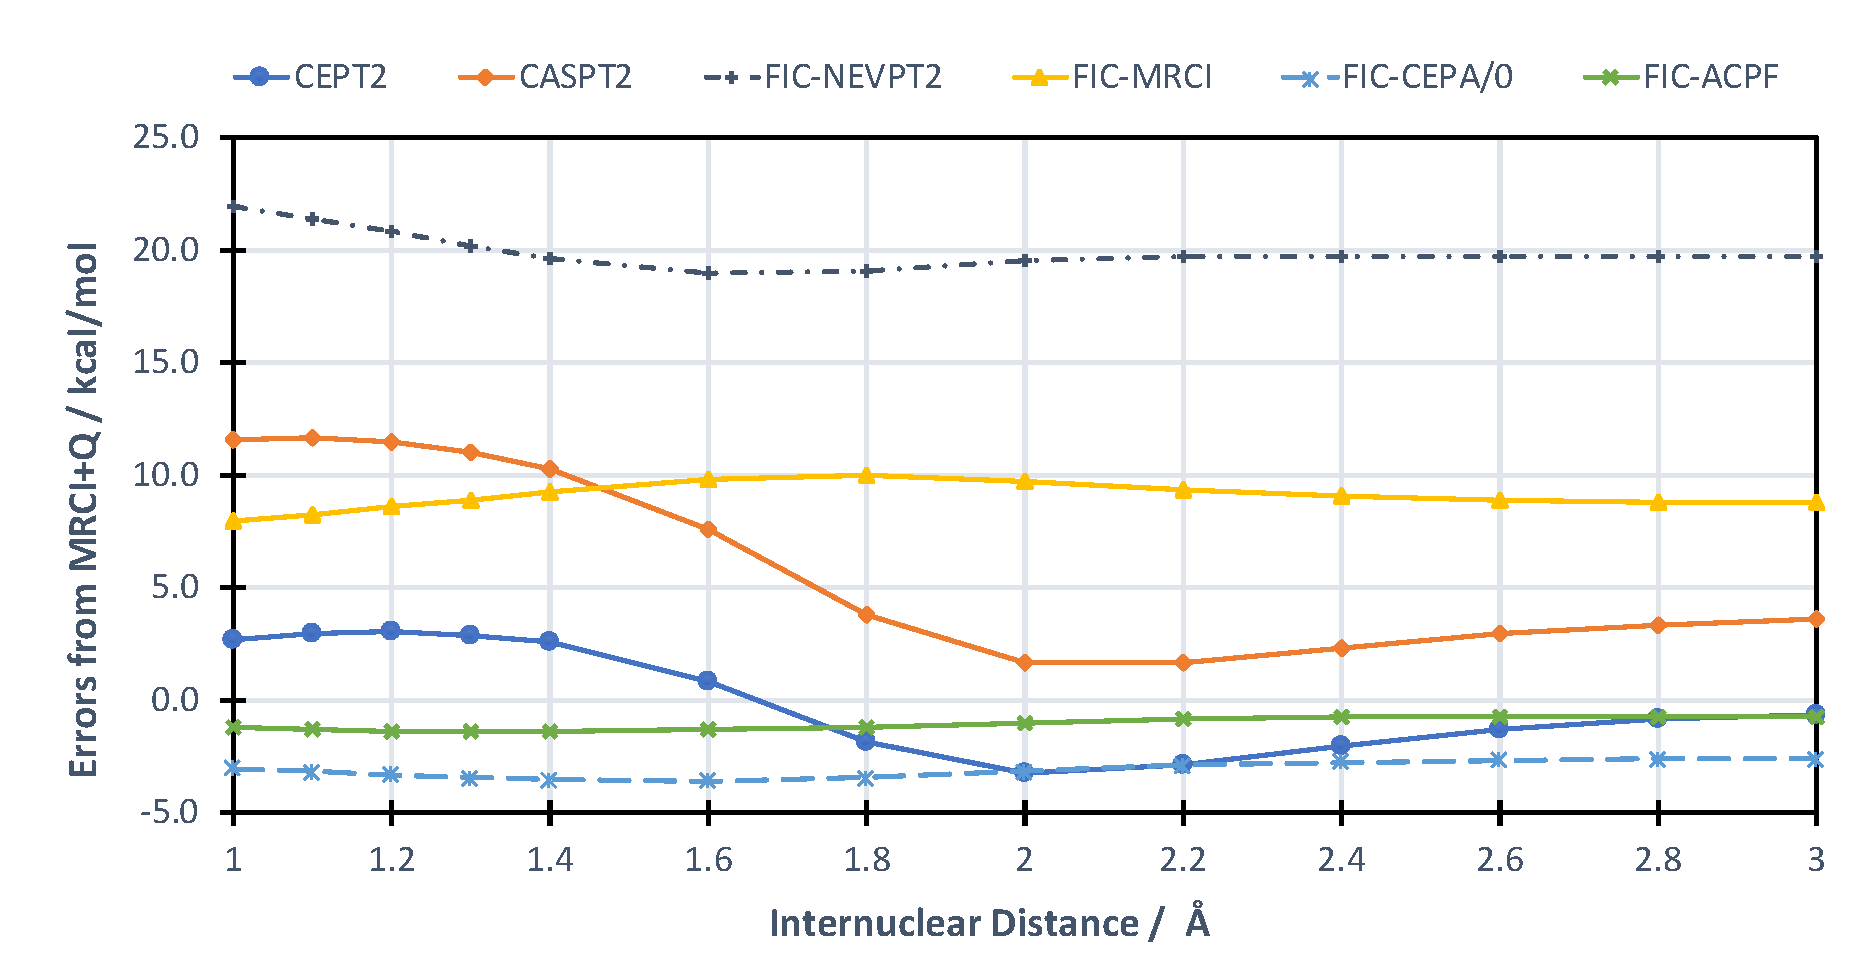
\includegraphics{CEPT-Comparison-CCSDT.pdf}}
    \caption{\label{fig:CEPT-Comparison}
      {
        %
        Deviations of canonical CEPT2 energy from those of MRCI+Q for $\text{N}_2$ with various internuclear distances with def2-QZVPP basis set.
        %
        1$s$ orbitals of nitrogen atoms were kept frozen while all the other orbitals were correlated.
        %
        All the 2$p$ orbitals were included in the active space leading to CAS(6$e$, 6$o$) treatment.
      }
    }
  \end{figure}
}

\newpage

{
  \begin{figure}[H]
    \scalebox{0.5}{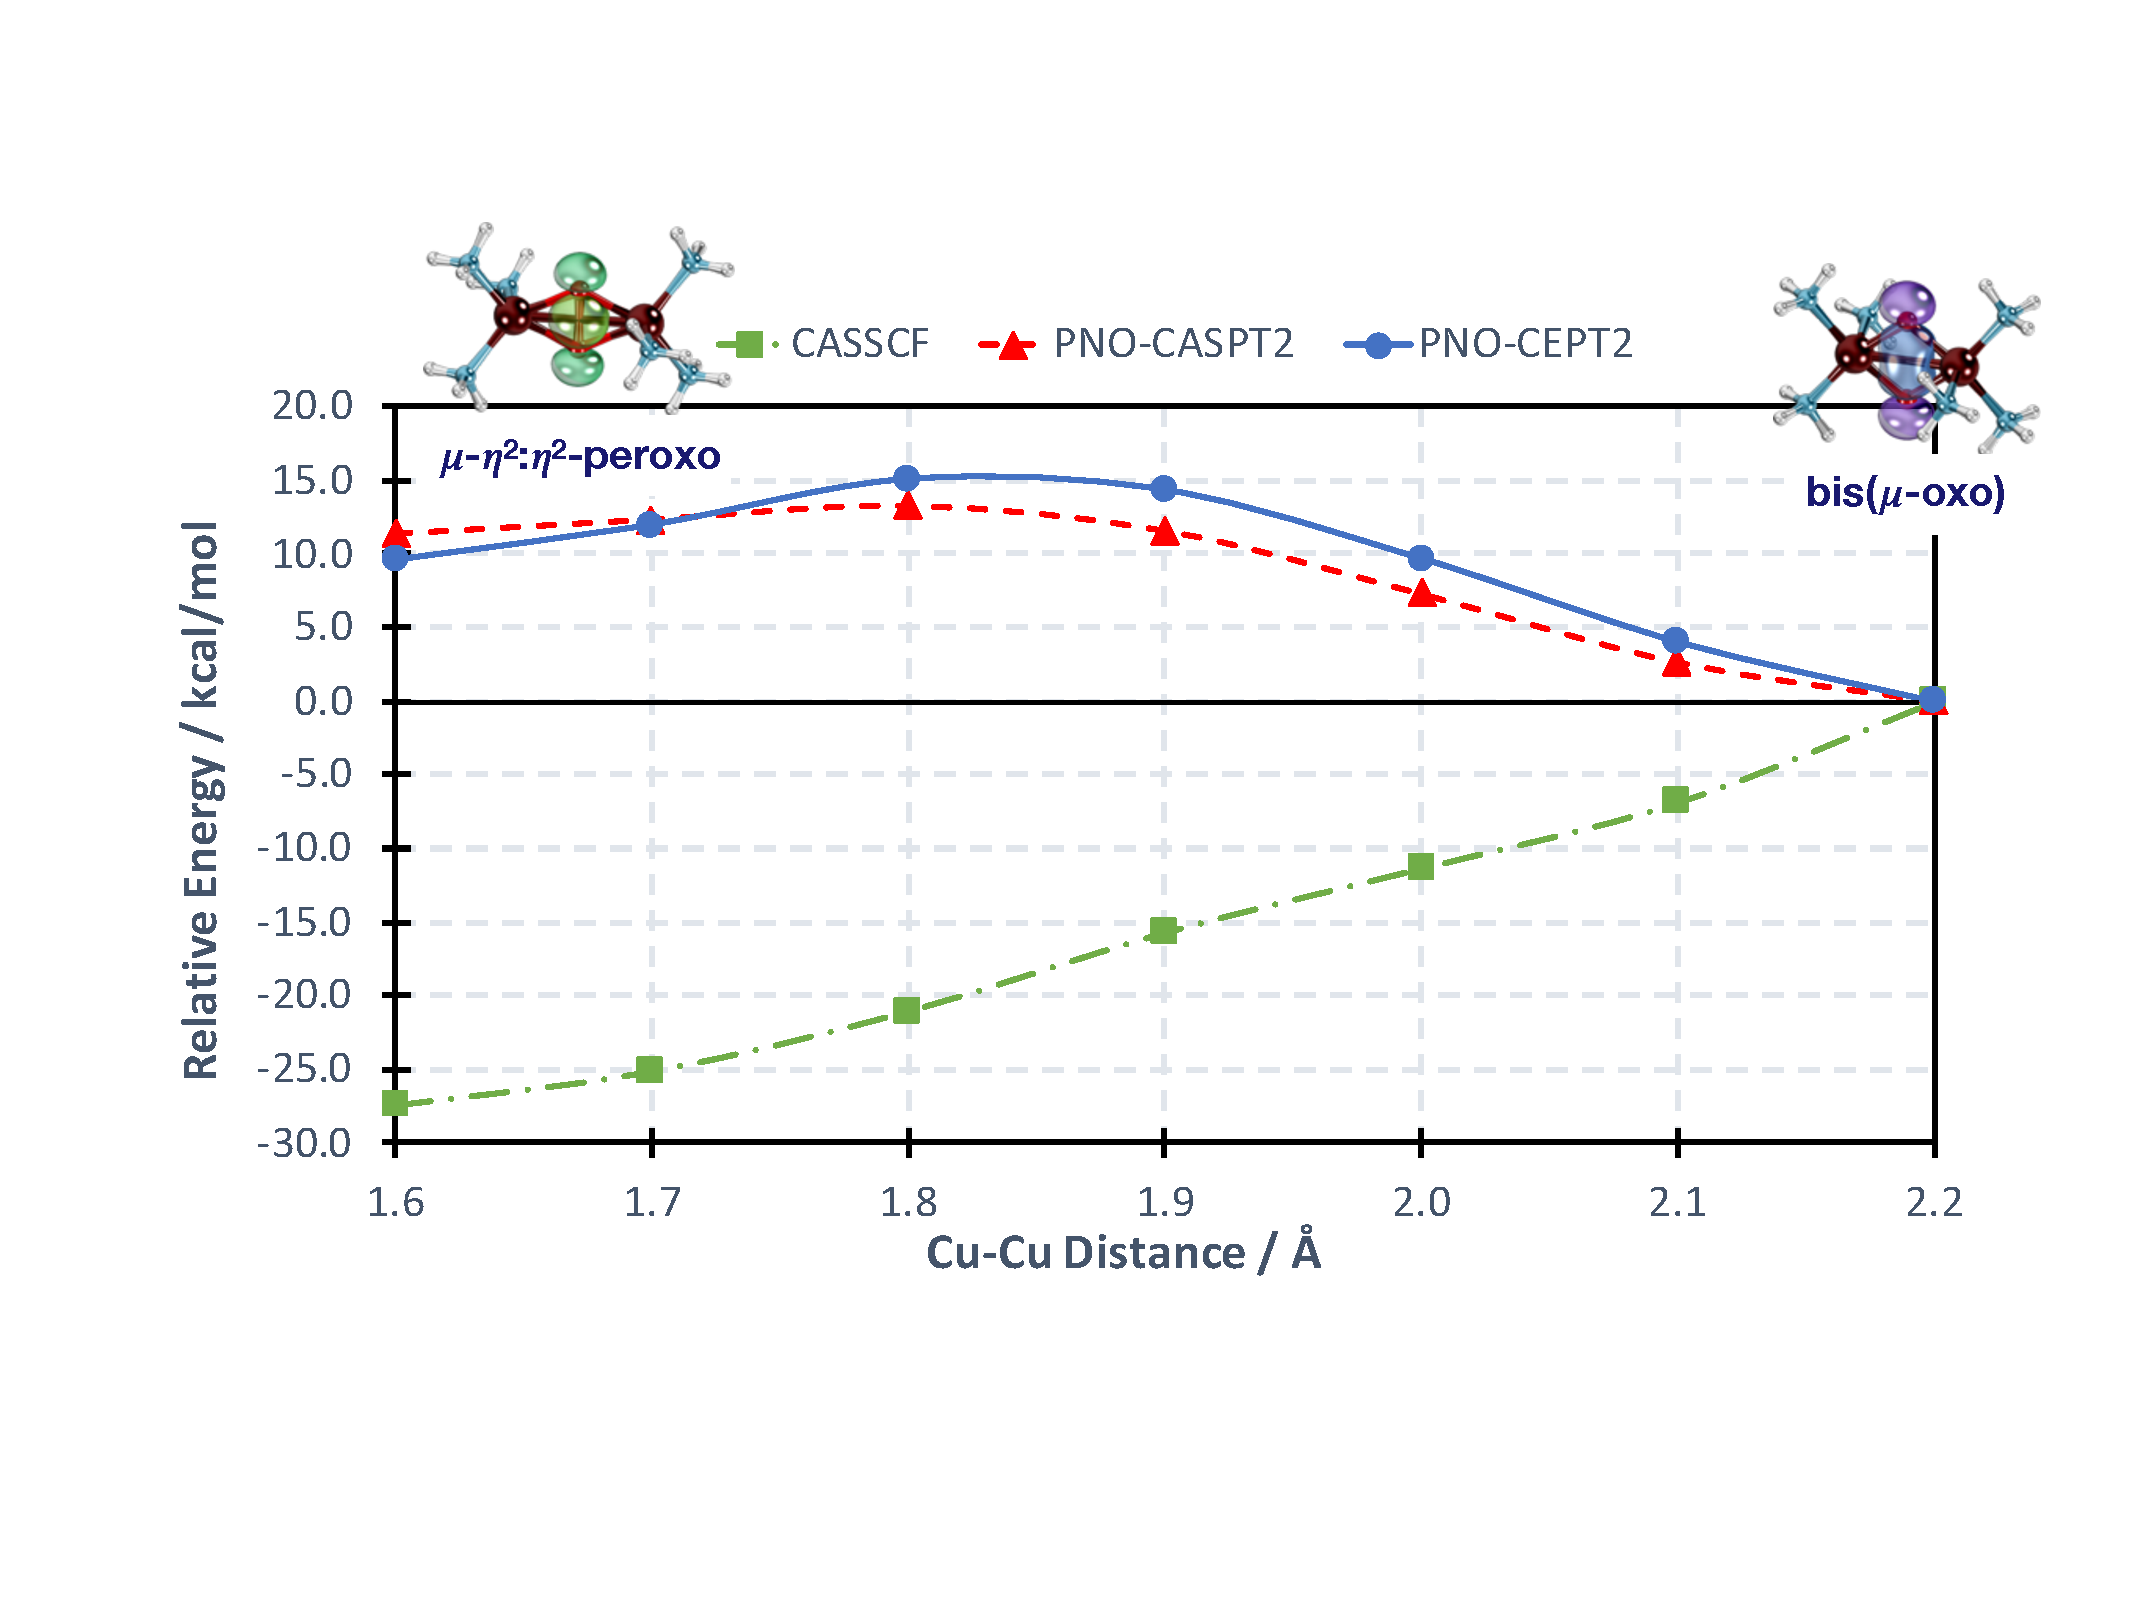
\includegraphics{Cu2O2-Isomerization-New.pdf}}
    \caption{\label{fig:CEPT-Cu2O2}
      {
        %
        Isomerization curves of [Cu${}_2$O${}_2$]$^{+2}$(NH${}_3$)${}_6$ calculated by PNO-CASPT2 and PNO-CEPT2 using def2-QZVPP (O, Mn) and def2-TZVPP (H, N) basis sets.
        %
        For the RI treatment, def2-TZVPP/C auxiliary basis was used.
        %
        All the O(1$s$), N(1$s$), Fe(1$s$, 2$s$, 2$p$) orbitals were kept frozen at the PNO-CASPT2/CEPT2 steps.
        %
        The active space is composed of O(2$p_x$, 2$p_y$, 3$p_x$, 3$p_y$) and Fe(3$d_{xy}$) thus leading to CAS(8$e$, 10$o$) treatment.
        %
        The PNO and weak-pair truncation thresholds were set to $5\times 10^{-1}$ and $1\times 10^{-5}$ Eh, respectively.
        %
        Total number of AO basis functions is 752.
      }
    }
  \end{figure}
}

\newpage

{
  \begin{figure}[H]
    \scalebox{0.4}{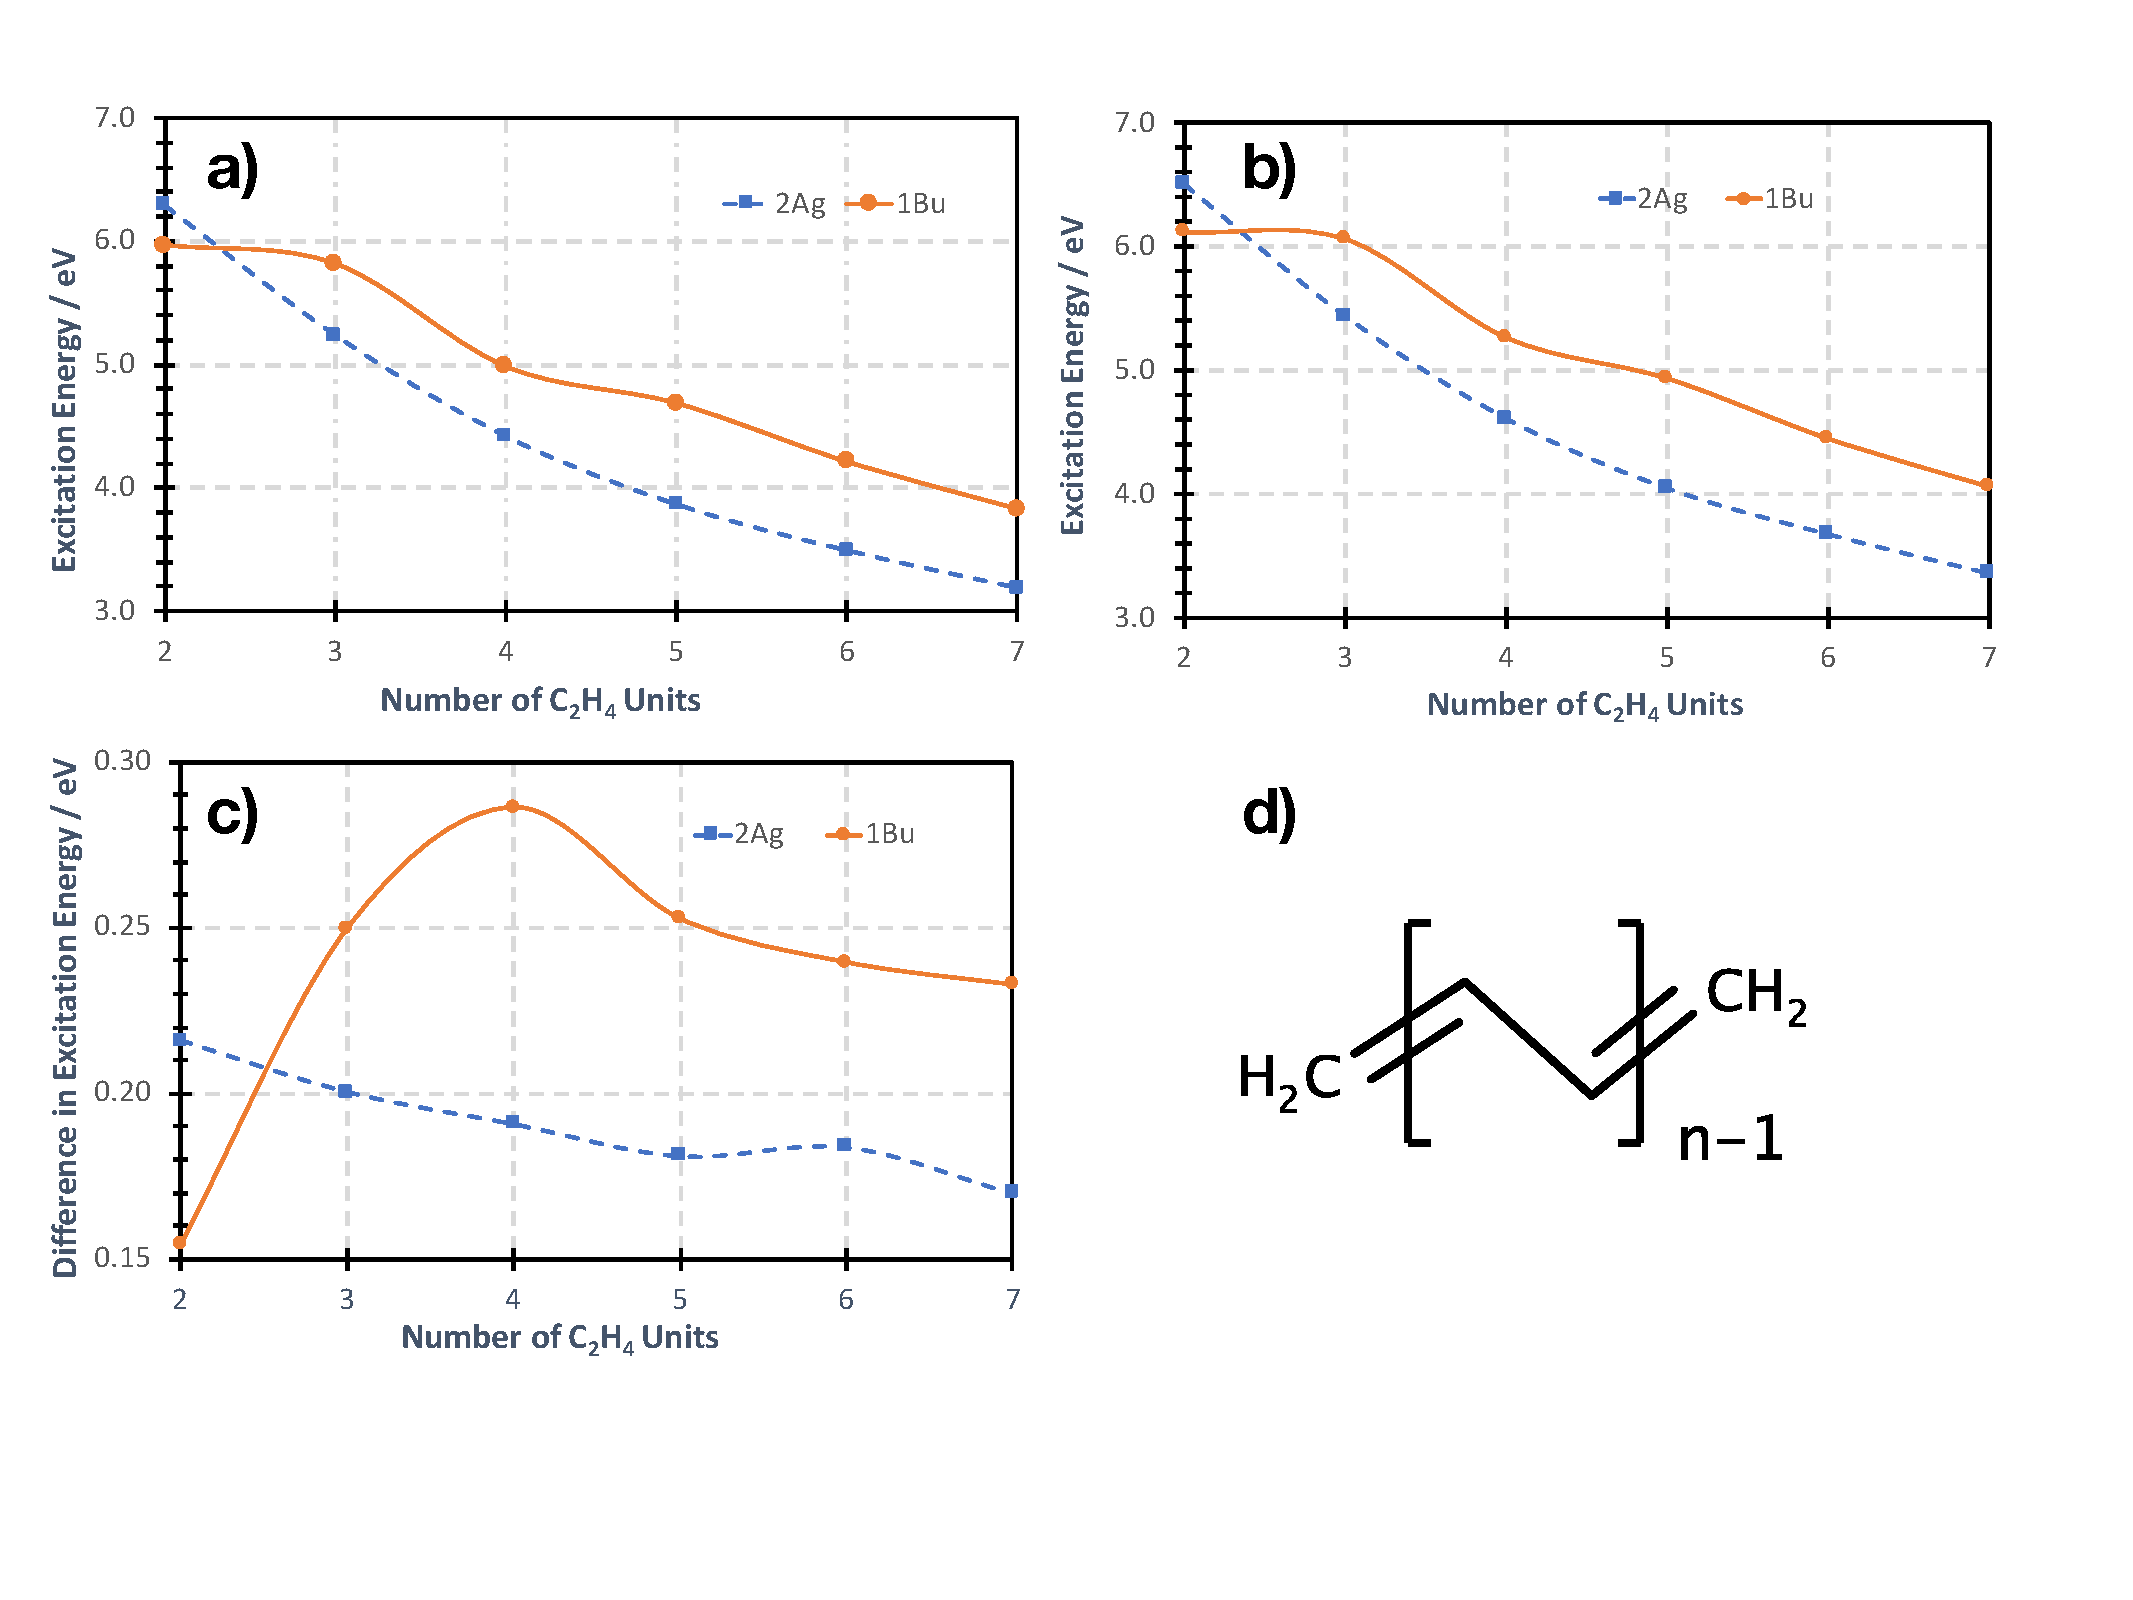
\includegraphics{Fig-Polyene.pdf}}
    \caption{\label{fig:Polyene}
      {
        %
        Vertical EEs for linear polyene, C${}_{2n}$H${}_{2n+2}$, calculated by a) canonical CASPT2 and the b) PNO-CEPT2 methods using PNO and weak-pair truncation thresholds set to $5.0\times 10^{-8}$ and $1.0\times 10^{-5}$ Eh, respectively.
        %
        Figure c) represents difference between canonical CASPT2 and PNO-CEPT2 EEs, EE(PNO-CEPT2)-EE(CASPT2), while Figure d) showing the general chemical formula for polyene chains.
        %
        The def2-TZVPP basis and def2-TZVPP/JK auxiliary basis sets were used.
        %
        All the C(1$s$) orbitals were kep frozen after the reference CASSCF calculation while C($2p_z$) orbitals were included in the active space, thus leading to CAS(2n $e$, 2n $o$) treatment.
        %
        No shifts were used in the zeroth-order Hamiltonian.
      }
    }
  \end{figure}
}

%%-NEW-NEW-NEW-NEW-NEW-NEW-NEW-NEW-NEW-NEW-NEW-NEW-NEW-NEW-NEW-NEW-NEW-NEW-NEW-NEW-NEW-NEW-NEW-NEW-NEW-NEW-NEW-NEW-NEW-NEW-NEW-NEW-NEW-NEW-NEW-NEW-NEW-NEW-NEW-NEW-NEW-NEW-NEW-NEW-NEW-NEW

\end{document}
